% ====================================================================
% PET NOTE -- companion to the analysis note (main_note.tex), split from it on 2026-10-12 at
% Joseph's request so the analysis note can accompany the scalar (GBDT) result on its own while
% the PET method development continues. Build: bash build_all.sh (a note-audience target).
% Shares preamble.tex, values.tex, publication.bib and the figure set.
% The PET sections and appendices are the analysis note's former appendices, moved verbatim
% except for cross-reference targets: references into the analysis note name its sections by
% title (\notesec, preamble.tex), because that note's numbering is a different build's.
% ====================================================================
\documentclass[11pt]{article}
\usepackage{authblk}
% Audience flags for the three builds (main_note / main_primer / main_paper). Each driver flips exactly one true after % Audience flags for the three builds (main_note / main_primer / main_paper). Each driver flips exactly one true after % Audience flags for the three builds (main_note / main_primer / main_paper). Each driver flips exactly one true after \input{preamble}; no section tests them today, but conditional content can hook on them.
\newif\ifNOTE
\newif\ifPRIMER
\newif\ifPAPER

% The analysis note (main_note) and its companion PET note (pet_note) are separate PDFs, so a reference from one into the other names the section by title: its number moves with every edit.
\newcommand{\notesec}[1]{the analysis note, \S``#1''}
\newcommand{\petsec}[1]{the companion PET note, \S``#1''}

\usepackage[margin=1in]{geometry}
\usepackage[T1]{fontenc}      % proper hyphenation + line breaking
\usepackage{amsmath,amssymb}
\usepackage{graphicx}
\usepackage[htt]{hyphenat}    % allow long \texttt{} paths to break across lines
\usepackage{microtype}        % character protrusion / font expansion: kills most overfull boxes
\emergencystretch=3em         % last-resort stretch so justified prose stays in the margin
\usepackage{float}      % enables [H] to pin figures inline
\usepackage{booktabs}
\usepackage{longtable}
\usepackage{siunitx}
\usepackage{enumitem}
\usepackage[hidelinks]{hyperref}
\usepackage{xcolor}
% Retraction marking. Repo convention is to STRIKE THROUGH rather than erase, so a reader who remembers a superseded number finds it struck rather than vanished (docs/orchestration/INDEX-retracted-and-superseded-values.md).
\usepackage[normalem]{ulem}
% Works in BOTH text and math mode: \mbox gives \sout an LR box to strike, and
% \ensuremath restores math for the (usual) numeric argument. Needed because most call sites are numbers already inside $...$, where \sout alone fails.
\newcommand{\dead}[1]{\mbox{\textcolor{gray}{\sout{\ensuremath{#1}}}}}
% Reviewer-comment macros. Defined HERE rather than in main_note.tex because all three external drivers input this file: they were note-local, and the paper build would have failed with Undefined control sequence the first time a commented paragraph was distilled into paper_body.tex. Definitions are verbatim from main_note.tex; xcolor is loaded above, which is what these need.
\newcommand{\bpn}[1]{\textcolor{blue}{\textbf{[BPN: #1]}}}
\newcommand{\jrb}[1]{\textcolor{violet}{\textbf{[JRB: #1]}}}
\newcommand{\gk}[1]{\textcolor{orange}{\textbf{[GK: #1]}}}
% biblatex + biber: clickable arXiv/doi links, "et al." rendering.
\usepackage[backend=biber, style=numeric-comp, sorting=none, giveninits=true,
            maxbibnames=3, minbibnames=1, doi=true, eprint=true, isbn=false, url=false]{biblatex}
\addbibresource{technote.bib}

% Public code repository: file paths cited throughout (drivers, event loop, UQ scripts) resolve against this tree.
\newcommand{\repourl}{https://github.com/josephbaileyy/MINERvA-OmniFold}
\newcommand{\repolink}{\href{\repourl}{\texttt{github.com/josephbaileyy/MINERvA-OmniFold}}}

% Figures live in the analysis directories; identical search path for every build.
\graphicspath{{figures/}}
% Vector-only: every figure now ships a .pdf twin, so we restrict the search to .pdf.  A missing vector then fails the build loudly instead of silently pulling in a stale raster .png.
\DeclareGraphicsExtensions{.pdf}

% Repository paths: \repopath{docs/orchestration/FOO-20260101-bar.md} sets the path in \texttt with a break opportunity after every "/" and "-", so a long path breaks inside a narrow column instead of running into the margin.
%
% WHY A MACRO RATHER THAN HAND-INSERTED \allowbreak, and it is not a style preference. The first fix for the margin overflow wrote the breaks into the source (docs/\allowbreak orchestration/\allowbreak AUDIT-...). That types identically and SILENTLY BROKE DISCOVERY: generate_manifest.py counts inbound references by matching the literal path, so seven records each lost a citation -- measured as inbound_count 11->10, 3->2, 26->25, 14->13, 10->9, 17->16 and 5->4. The macro keeps the argument a literal, greppable path and inserts the breaks at typeset time instead.
% \path{} was also tried: it breaks too reluctantly and still overflowed. NOTE: the argument may not contain "_" (it would need catcode surgery); no path routed here does, and the one that does is written with \texttt{...\_...} directly.
\makeatletter
\newcommand{\mnv@stop}{}
\newcommand{\repopath}[1]{\texttt{\mnv@brk#1\mnv@stop}}
\def\mnv@brk#1{%
  \ifx\mnv@stop#1\else
    #1%
    \ifx#1/\allowbreak\fi
    \ifx#1-\allowbreak\fi
    \expandafter\mnv@brk
  \fi}
\makeatother

% --- notation macros ---
\newcommand{\pT}{p_{T}}
\newcommand{\pPar}{p_{\parallel}}
\newcommand{\Eavail}{E_{\mathrm{avail}}}
\newcommand{\TODO}[1]{\textcolor{red}{[TODO: #1]}}
% macros used by the statistical-methods appendix
\newcommand{\dpT}{\Delta\pT}
\newcommand{\xsec}{\mathrm{xs}}
\newcommand{\ours}{\text{ours}}
\newcommand{\paper}{\text{paper}}
\newcommand{\CV}{\text{CV}}
\newcommand{\boot}{\text{boot}}
\newcommand{\stat}{\text{stat}}
\newcommand{\syst}{\text{syst}}
\newcommand{\ML}{\text{ML}}
\newcommand{\tot}{\text{tot}}
\newcommand{\T}{^{\!\top}}
\newcommand{\diag}{\mathrm{diag}}
\newcommand{\Tr}{\mathrm{Tr}}

% Note register round n2, N2-1 (director rulings 2026-10-26): \recentry{<tag>} prints a records entry's number (R1.<n>), so the posted note cites a records entry by number instead of by its internal tag. The numbers are generated from app_provenance.tex by `check_note_records.py entry-numbers`; build_all.sh fails if the file is stale (before any build or export) or if a number differs from the records build's own label (after it).
\input{records_entry_numbers}
; no section tests them today, but conditional content can hook on them.
\newif\ifNOTE
\newif\ifPRIMER
\newif\ifPAPER

% The analysis note (main_note) and its companion PET note (pet_note) are separate PDFs, so a reference from one into the other names the section by title: its number moves with every edit.
\newcommand{\notesec}[1]{the analysis note, \S``#1''}
\newcommand{\petsec}[1]{the companion PET note, \S``#1''}

\usepackage[margin=1in]{geometry}
\usepackage[T1]{fontenc}      % proper hyphenation + line breaking
\usepackage{amsmath,amssymb}
\usepackage{graphicx}
\usepackage[htt]{hyphenat}    % allow long \texttt{} paths to break across lines
\usepackage{microtype}        % character protrusion / font expansion: kills most overfull boxes
\emergencystretch=3em         % last-resort stretch so justified prose stays in the margin
\usepackage{float}      % enables [H] to pin figures inline
\usepackage{booktabs}
\usepackage{longtable}
\usepackage{siunitx}
\usepackage{enumitem}
\usepackage[hidelinks]{hyperref}
\usepackage{xcolor}
% Retraction marking. Repo convention is to STRIKE THROUGH rather than erase, so a reader who remembers a superseded number finds it struck rather than vanished (docs/orchestration/INDEX-retracted-and-superseded-values.md).
\usepackage[normalem]{ulem}
% Works in BOTH text and math mode: \mbox gives \sout an LR box to strike, and
% \ensuremath restores math for the (usual) numeric argument. Needed because most call sites are numbers already inside $...$, where \sout alone fails.
\newcommand{\dead}[1]{\mbox{\textcolor{gray}{\sout{\ensuremath{#1}}}}}
% Reviewer-comment macros. Defined HERE rather than in main_note.tex because all three external drivers input this file: they were note-local, and the paper build would have failed with Undefined control sequence the first time a commented paragraph was distilled into paper_body.tex. Definitions are verbatim from main_note.tex; xcolor is loaded above, which is what these need.
\newcommand{\bpn}[1]{\textcolor{blue}{\textbf{[BPN: #1]}}}
\newcommand{\jrb}[1]{\textcolor{violet}{\textbf{[JRB: #1]}}}
\newcommand{\gk}[1]{\textcolor{orange}{\textbf{[GK: #1]}}}
% biblatex + biber: clickable arXiv/doi links, "et al." rendering.
\usepackage[backend=biber, style=numeric-comp, sorting=none, giveninits=true,
            maxbibnames=3, minbibnames=1, doi=true, eprint=true, isbn=false, url=false]{biblatex}
\addbibresource{technote.bib}

% Public code repository: file paths cited throughout (drivers, event loop, UQ scripts) resolve against this tree.
\newcommand{\repourl}{https://github.com/josephbaileyy/MINERvA-OmniFold}
\newcommand{\repolink}{\href{\repourl}{\texttt{github.com/josephbaileyy/MINERvA-OmniFold}}}

% Figures live in the analysis directories; identical search path for every build.
\graphicspath{{figures/}}
% Vector-only: every figure now ships a .pdf twin, so we restrict the search to .pdf.  A missing vector then fails the build loudly instead of silently pulling in a stale raster .png.
\DeclareGraphicsExtensions{.pdf}

% Repository paths: \repopath{docs/orchestration/FOO-20260101-bar.md} sets the path in \texttt with a break opportunity after every "/" and "-", so a long path breaks inside a narrow column instead of running into the margin.
%
% WHY A MACRO RATHER THAN HAND-INSERTED \allowbreak, and it is not a style preference. The first fix for the margin overflow wrote the breaks into the source (docs/\allowbreak orchestration/\allowbreak AUDIT-...). That types identically and SILENTLY BROKE DISCOVERY: generate_manifest.py counts inbound references by matching the literal path, so seven records each lost a citation -- measured as inbound_count 11->10, 3->2, 26->25, 14->13, 10->9, 17->16 and 5->4. The macro keeps the argument a literal, greppable path and inserts the breaks at typeset time instead.
% \path{} was also tried: it breaks too reluctantly and still overflowed. NOTE: the argument may not contain "_" (it would need catcode surgery); no path routed here does, and the one that does is written with \texttt{...\_...} directly.
\makeatletter
\newcommand{\mnv@stop}{}
\newcommand{\repopath}[1]{\texttt{\mnv@brk#1\mnv@stop}}
\def\mnv@brk#1{%
  \ifx\mnv@stop#1\else
    #1%
    \ifx#1/\allowbreak\fi
    \ifx#1-\allowbreak\fi
    \expandafter\mnv@brk
  \fi}
\makeatother

% --- notation macros ---
\newcommand{\pT}{p_{T}}
\newcommand{\pPar}{p_{\parallel}}
\newcommand{\Eavail}{E_{\mathrm{avail}}}
\newcommand{\TODO}[1]{\textcolor{red}{[TODO: #1]}}
% macros used by the statistical-methods appendix
\newcommand{\dpT}{\Delta\pT}
\newcommand{\xsec}{\mathrm{xs}}
\newcommand{\ours}{\text{ours}}
\newcommand{\paper}{\text{paper}}
\newcommand{\CV}{\text{CV}}
\newcommand{\boot}{\text{boot}}
\newcommand{\stat}{\text{stat}}
\newcommand{\syst}{\text{syst}}
\newcommand{\ML}{\text{ML}}
\newcommand{\tot}{\text{tot}}
\newcommand{\T}{^{\!\top}}
\newcommand{\diag}{\mathrm{diag}}
\newcommand{\Tr}{\mathrm{Tr}}

% Note register round n2, N2-1 (director rulings 2026-10-26): \recentry{<tag>} prints a records entry's number (R1.<n>), so the posted note cites a records entry by number instead of by its internal tag. The numbers are generated from app_provenance.tex by `check_note_records.py entry-numbers`; build_all.sh fails if the file is stale (before any build or export) or if a number differs from the records build's own label (after it).
% GENERATED by `python3 check_note_records.py entry-numbers` from app_provenance.tex; never edit by hand.
% The number of every full-width records entry, as main_records.tex's label hook numbers it, so the
% posted note can cite an entry as \recentry{<tag>} without reading the records build.
% `entry-numbers --check` fails if this file is stale; `entry-numbers --check-aux` (build_all.sh, after
% the records build) fails if a number differs from main_records.aux.
\makeatletter
\providecommand{\recentry}[1]{\@ifundefined{recentry@#1}{\PackageError{records_entry_numbers}{no
  records entry is numbered for the tag #1}{Regenerate with check_note_records.py entry-numbers.}}%
  {\@nameuse{recentry@#1}}}
\@namedef{recentry@coverage-fixed-truth}{R1.1}
\@namedef{recentry@coverage-toys}{R1.2}
\@namedef{recentry@flux-repair}{R1.3}
\@namedef{recentry@z-cv-record}{R1.4}
\@namedef{recentry@joint-5d}{R1.5}
\@namedef{recentry@variance-sources}{R1.6}
\@namedef{recentry@negweight-hpss}{R1.7}
\@namedef{recentry@oi6-oi8-oi126}{R1.8}
\@namedef{recentry@fps-battery}{R1.9}
\@namedef{recentry@z-projection}{R1.10}
\@namedef{recentry@z-conditioning}{R1.11}
\@namedef{recentry@2d-central-value}{R1.12}
\@namedef{recentry@flux-index}{R1.13}
\@namedef{recentry@response-diagnostic}{R1.14}
\@namedef{recentry@rank-inversion}{R1.15}
\@namedef{recentry@july-sweep}{R1.16}
\@namedef{recentry@bkg-mode-elimination}{R1.17}
\@namedef{recentry@mp5-truth-axis}{R1.18}
\makeatother

; no section tests them today, but conditional content can hook on them.
\newif\ifNOTE
\newif\ifPRIMER
\newif\ifPAPER

% The analysis note (main_note) and its companion PET note (pet_note) are separate PDFs, so a reference from one into the other names the section by title: its number moves with every edit.
\newcommand{\notesec}[1]{the analysis note, \S``#1''}
\newcommand{\petsec}[1]{the companion PET note, \S``#1''}

\usepackage[margin=1in]{geometry}
\usepackage[T1]{fontenc}      % proper hyphenation + line breaking
\usepackage{amsmath,amssymb}
\usepackage{graphicx}
\usepackage[htt]{hyphenat}    % allow long \texttt{} paths to break across lines
\usepackage{microtype}        % character protrusion / font expansion: kills most overfull boxes
\emergencystretch=3em         % last-resort stretch so justified prose stays in the margin
\usepackage{float}      % enables [H] to pin figures inline
\usepackage{booktabs}
\usepackage{longtable}
\usepackage{siunitx}
\usepackage{enumitem}
\usepackage[hidelinks]{hyperref}
\usepackage{xcolor}
% Retraction marking. Repo convention is to STRIKE THROUGH rather than erase, so a reader who remembers a superseded number finds it struck rather than vanished (docs/orchestration/INDEX-retracted-and-superseded-values.md).
\usepackage[normalem]{ulem}
% Works in BOTH text and math mode: \mbox gives \sout an LR box to strike, and
% \ensuremath restores math for the (usual) numeric argument. Needed because most call sites are numbers already inside $...$, where \sout alone fails.
\newcommand{\dead}[1]{\mbox{\textcolor{gray}{\sout{\ensuremath{#1}}}}}
% Reviewer-comment macros. Defined HERE rather than in main_note.tex because all three external drivers input this file: they were note-local, and the paper build would have failed with Undefined control sequence the first time a commented paragraph was distilled into paper_body.tex. Definitions are verbatim from main_note.tex; xcolor is loaded above, which is what these need.
\newcommand{\bpn}[1]{\textcolor{blue}{\textbf{[BPN: #1]}}}
\newcommand{\jrb}[1]{\textcolor{violet}{\textbf{[JRB: #1]}}}
\newcommand{\gk}[1]{\textcolor{orange}{\textbf{[GK: #1]}}}
% biblatex + biber: clickable arXiv/doi links, "et al." rendering.
\usepackage[backend=biber, style=numeric-comp, sorting=none, giveninits=true,
            maxbibnames=3, minbibnames=1, doi=true, eprint=true, isbn=false, url=false]{biblatex}
\addbibresource{technote.bib}

% Public code repository: file paths cited throughout (drivers, event loop, UQ scripts) resolve against this tree.
\newcommand{\repourl}{https://github.com/josephbaileyy/MINERvA-OmniFold}
\newcommand{\repolink}{\href{\repourl}{\texttt{github.com/josephbaileyy/MINERvA-OmniFold}}}

% Figures live in the analysis directories; identical search path for every build.
\graphicspath{{figures/}}
% Vector-only: every figure now ships a .pdf twin, so we restrict the search to .pdf.  A missing vector then fails the build loudly instead of silently pulling in a stale raster .png.
\DeclareGraphicsExtensions{.pdf}

% Repository paths: \repopath{docs/orchestration/FOO-20260101-bar.md} sets the path in \texttt with a break opportunity after every "/" and "-", so a long path breaks inside a narrow column instead of running into the margin.
%
% WHY A MACRO RATHER THAN HAND-INSERTED \allowbreak, and it is not a style preference. The first fix for the margin overflow wrote the breaks into the source (docs/\allowbreak orchestration/\allowbreak AUDIT-...). That types identically and SILENTLY BROKE DISCOVERY: generate_manifest.py counts inbound references by matching the literal path, so seven records each lost a citation -- measured as inbound_count 11->10, 3->2, 26->25, 14->13, 10->9, 17->16 and 5->4. The macro keeps the argument a literal, greppable path and inserts the breaks at typeset time instead.
% \path{} was also tried: it breaks too reluctantly and still overflowed. NOTE: the argument may not contain "_" (it would need catcode surgery); no path routed here does, and the one that does is written with \texttt{...\_...} directly.
\makeatletter
\newcommand{\mnv@stop}{}
\newcommand{\repopath}[1]{\texttt{\mnv@brk#1\mnv@stop}}
\def\mnv@brk#1{%
  \ifx\mnv@stop#1\else
    #1%
    \ifx#1/\allowbreak\fi
    \ifx#1-\allowbreak\fi
    \expandafter\mnv@brk
  \fi}
\makeatother

% --- notation macros ---
\newcommand{\pT}{p_{T}}
\newcommand{\pPar}{p_{\parallel}}
\newcommand{\Eavail}{E_{\mathrm{avail}}}
\newcommand{\TODO}[1]{\textcolor{red}{[TODO: #1]}}
% macros used by the statistical-methods appendix
\newcommand{\dpT}{\Delta\pT}
\newcommand{\xsec}{\mathrm{xs}}
\newcommand{\ours}{\text{ours}}
\newcommand{\paper}{\text{paper}}
\newcommand{\CV}{\text{CV}}
\newcommand{\boot}{\text{boot}}
\newcommand{\stat}{\text{stat}}
\newcommand{\syst}{\text{syst}}
\newcommand{\ML}{\text{ML}}
\newcommand{\tot}{\text{tot}}
\newcommand{\T}{^{\!\top}}
\newcommand{\diag}{\mathrm{diag}}
\newcommand{\Tr}{\mathrm{Tr}}

% Note register round n2, N2-1 (director rulings 2026-10-26): \recentry{<tag>} prints a records entry's number (R1.<n>), so the posted note cites a records entry by number instead of by its internal tag. The numbers are generated from app_provenance.tex by `check_note_records.py entry-numbers`; build_all.sh fails if the file is stale (before any build or export) or if a number differs from the records build's own label (after it).
% GENERATED by `python3 check_note_records.py entry-numbers` from app_provenance.tex; never edit by hand.
% The number of every full-width records entry, as main_records.tex's label hook numbers it, so the
% posted note can cite an entry as \recentry{<tag>} without reading the records build.
% `entry-numbers --check` fails if this file is stale; `entry-numbers --check-aux` (build_all.sh, after
% the records build) fails if a number differs from main_records.aux.
\makeatletter
\providecommand{\recentry}[1]{\@ifundefined{recentry@#1}{\PackageError{records_entry_numbers}{no
  records entry is numbered for the tag #1}{Regenerate with check_note_records.py entry-numbers.}}%
  {\@nameuse{recentry@#1}}}
\@namedef{recentry@coverage-fixed-truth}{R1.1}
\@namedef{recentry@coverage-toys}{R1.2}
\@namedef{recentry@flux-repair}{R1.3}
\@namedef{recentry@z-cv-record}{R1.4}
\@namedef{recentry@joint-5d}{R1.5}
\@namedef{recentry@variance-sources}{R1.6}
\@namedef{recentry@negweight-hpss}{R1.7}
\@namedef{recentry@oi6-oi8-oi126}{R1.8}
\@namedef{recentry@fps-battery}{R1.9}
\@namedef{recentry@z-projection}{R1.10}
\@namedef{recentry@z-conditioning}{R1.11}
\@namedef{recentry@2d-central-value}{R1.12}
\@namedef{recentry@flux-index}{R1.13}
\@namedef{recentry@response-diagnostic}{R1.14}
\@namedef{recentry@rank-inversion}{R1.15}
\@namedef{recentry@july-sweep}{R1.16}
\@namedef{recentry@bkg-mode-elimination}{R1.17}
\@namedef{recentry@mp5-truth-axis}{R1.18}
\makeatother


\NOTEtrue
% ====================================================================
% values.tex --- SINGLE SOURCE OF TRUTH for every headline number that
% recurs across the build (abstract / executive summary / body section).
% Edit a result HERE and it updates in all three PDFs.
% Numbers that appear exactly once (deep in a section, a table,
% or App. B) are NOT macroized here -- they cannot drift, so they stay inline
% at their single site.
%
% Convention: cross sections carry their full value+exponent so \SI expands
% cleanly (e.g. \SI{\sigTwoD}{cm^2/nucleon}); ratios/percentages/significances
% are bare numbers (e.g. \SI{\uqMedian}{\percent}, $\ratioTot$).
% ====================================================================

% --- 2D reproduction (the demonstrator) ---
% CENTRAL VALUE SWITCHED 2026-10-11 (Joseph): the quoted 2D central value is now the LightGBM seed-42
% matched CV of the systematic sweep, uq/2d_xsec_MEFHC_5iter_lgbm_uni_full_CV.root, sha256
% 4f5a1b6d44b9e7212b233650bb00bfb626ae65461e3bf8033cd67866dbd7eb2c, no longer the exact-split
% 2d_crossSection_omnifold_MEFHC_5iter.root (142a45b0...). Decision record:
% docs/publication/DECISION-20261011-joseph-2d-central-lightgbm-seed42.md. Every macro below that depends
% on the central value was re-measured by the SAME committed producers at e1216e9c (saul login05, ROOT
% 6.28/12); receipts in docs/orchestration/receipts/2d-lgbm42-20261011/ (SHA256SUMS). Control: the same
% producers on the exact-split file reproduce 3.661 and 0.089/0.598. The provenance blocks below describe
% the 2026-08-21 receipts for the exact-split values (kept as history); the values printed are the new ones,
% each with its new receipt in its trailing comment.
% PROVENANCE, ADDED 2026-08-21 (OI-130). These three were the HARD CORE of the OI-130
% enumeration: of 71 macros they were the only ones naming NO backing artifact anywhere, even
% under the generous bound -- which makes them UNBINDABLE BY CONSTRUCTION, since no hash-binding,
% freeze gate or receipt check can fire on a macro that cites no path. They are the most-quoted
% numbers in the note, so that was the worst place for the gap to be.
%   PRODUCER  2d-unfolding/agreement_windows_receipt.py
%   RECEIPT   docs/orchestration/receipts/RECEIPT-2d-agreement-windows-20260821.json
%   RUN       saul, ROOT 6.28/12, at git 5996eb29
%   ARTIFACTS ours  hXSec2D             from 2d-unfolding/2d_crossSection_omnifold_MEFHC_5iter.root
%                                       sha256 142a45b0efc753d91e95376c28ac3f6a477d582014a919e49d6d71079a127fd5
%             paper pt_pl_cross_section  from minerva_paper_anc/cov_ptpl_minerva_inclusive_6GeV.root
%                                       sha256 6c6dce72050bb8f128fab8e286349b250bc60d1c767e162bf15a0f009f3573e3
%   MEASURED  integral ours 3.0733e-38; paper 3.0390e-38; ratio 1.0113
% THE TOTAL IS AN INTEGRAL, NOT A SUM OF BIN CONTENTS, and getting that wrong is easy here: these
% histograms hold d2sigma/(dpT dp_par), so the bin-area Jacobian is required. Measured without it,
% the sums came out 12.14x these values -- THE SAME FACTOR ON BOTH FILES -- while the RATIO still
% reproduced, because the Jacobian cancels. A ratio agreeing is not evidence that its operands do;
% the receipt keeps both numbers so nobody repeats it.
% STILL NOT ESTABLISHED: that this producer is the method that ORIGINALLY produced these three, and
% both artifacts live on PURGEABLE SCRATCH and are untracked, so this closes the CITATION gap and
% not the DURABILITY one (OI-130's class, and OI-75 for the same shape elsewhere).
\newcommand{\sigTwoD}{3.069e-38}      % RE-2 E_R/Q_R 3.06874e-38 (re2-integration/ledger.tsv row m-sigTwoD); was 3.073e-38: our 2D total; integral 3.0730e-38 (LightGBM seed 42; exact-split was 3.0733e-38), RECEIPT-2d-agreement-windows-lgbm42-20261011.json
\newcommand{\sigTwoDpaper}{3.039e-38} % published 2D total; integral 3.0390e-38, receipt above
\newcommand{\ratioTot}{1.010}         % RE-2 E_R/Q_R 1.00978 (re2-integration/ledger.tsv row m-ratioTot); was 1.011: sigma_tot ours/paper; integral ratio 1.0112 (exact-split was 1.0113), lgbm42 receipt
% PROVENANCE FOR THE NEXT FOUR MACROS -- RESOLVED 2026-08-21, AND THE HISTORY MATTERS.
% \medianBinRatio, \binsFive, \binsTen and \binsTwenty had NO committed producing script
% (OI-130). They were suppressed from all three deliverables on 2026-08-21 and are RESTORED
% here only because an authorized producer now attests them.
%   PRODUCER  2d-unfolding/agreement_windows_receipt.py
%   RECEIPT   docs/orchestration/receipts/RECEIPT-2d-agreement-windows-20260821.json
%   RUN       saul login34, ROOT 6.28/12, at git a3a4d3d1
%   MASK      205 of 224 bins, DERIVED as the positive diagonal of the paper ancillary's
%             StatOnlyCovariance on its own 224-bin global grid -- the same predicate
%             compare_to_paper_fullcov.py uses for its chi^2 ndf. The count is ASSERTED to be
%             205 and the producer exits 3 on any other value.
%   DENOM     205 of 205; ZERO bins excluded for a non-positive paper value, so the
%             denominator rule never bit and cannot be the source of the agreement.
%   INPUTS    ours  hXSec2D             from 2d_crossSection_omnifold_MEFHC_5iter.root
%                                       sha256 142a45b0efc753d91e95376c28ac3f6a477d582014a919e49d6d71079a127fd5
%             paper pt_pl_cross_section  from minerva_paper_anc/cov_ptpl_minerva_inclusive_6GeV.root
%                                       sha256 6c6dce72050bb8f128fab8e286349b250bc60d1c767e162bf15a0f009f3573e3
%   MEASURED  median 1.0064; 159/205 = 77.6 %; 193/205 = 94.1 %; 202/205 = 98.5 %
% ALL FOUR REPRODUCE THE PREVIOUSLY UNATTESTED VALUES EXACTLY. The producer was not aimed at
% them -- its receipt predeclares, in a field written before the run, that it attempts no
% reproduction and that a difference would be a finding.
% \medianBinRatio KEEPS ITS THREE-DECIMAL FORM: the receipt measures 1.0064 and 1.006 is that
% number at the precision the note has always printed. Changing the displayed precision would
% be a new editorial claim, not a restoration; the full value lives in the receipt.
% WHAT IS STILL NOT ESTABLISHED, and do not let the agreement blur it: this is not shown to be
% the method that ORIGINALLY produced these four. That provenance remains unrecoverable. OI-130's
% finding -- that no committed script reproduced the trio -- was TRUE OF THE TREE AS IT STOOD and
% stopped being true only when the producer landed.
% NOT THE PRODUCER, and the reason is worth keeping: 2d-unfolding/compare_to_paper_interior.py
% computes 5/10/20 % windows but masks to the STRICT INTERIOR (interior_mask(), pt_hi/pz_lo <=
% tan(20 deg)) intersected with the reported mask, so its denominators are SMALLER than 205
% (the audit's re-run reports 185/179/171/162/152/141). `git log --follow` puts that interior
% mask in the initial commit (d3239355), so no committed version of IT ever produced these.
% Any future change to these four goes through the producer and a fresh receipt.
\newcommand{\medianBinRatio}{1.005}   % RE-2 E_R/Q_R 1.0054 (re2-integration/ledger.tsv row m-medianBinRatio); was 1.008: median per-bin ratio ours/paper; lgbm42 receipt measures 1.0081 (exact-split 1.0064)
\newcommand{\binsFive}{86.8}          % RE-2 E_R/Q_R 86.8 (re2-integration/ledger.tsv row m-binsFive); was 82.9: percent of bins within 5%; 170/205, lgbm42 receipt (exact-split 77.6)
\newcommand{\binsTen}{95.1}           % RE-2 E_R/Q_R 95.1 (re2-integration/ledger.tsv row m-binsTen); was 95.6: within 10%; 196/205, lgbm42 receipt (exact-split 94.1)
\newcommand{\binsTwenty}{99.0}        % within 20%; 203/205, lgbm42 receipt (exact-split 98.5)
\newcommand{\pullMean}{0.060}         % RE-2 E_R/Q_R 0.06 (re2-integration/ledger.tsv row m-pullMean); was 0.074: chi2_lgbm42_paperonly.txt (exact-split 0.089)
\newcommand{\pullRMS}{0.535}          % RE-2 E_R/Q_R 0.535 (re2-integration/ledger.tsv row m-pullRMS); was 0.564: chi2_lgbm42_paperonly.txt (exact-split 0.598)
\newcommand{\pullRMSr}{0.54}          % RE-2 E_R/Q_R 0.535 (re2-integration/ledger.tsv row m-pullRMSr); was 0.56: rounded, for prose
% FPS containment (Agent C WS1 statistical-validation repair, 2026-07-16):
% split-sample +/-1sigma truth-containment against an independent fixed NPZ truth.
% The estimator seed is fixed, so this diagnoses the statistical closure-toy
% stream, not the full adopted band. No aggregate binomial error is quoted.
\newcommand{\covFPS}{68.67}
\newcommand{\covNominal}{68.27}                              % Gaussian nominal
\newcommand{\covFPSanalytic}{77.6}   % FPS variant-A (scalar uq_cov_stat_fps.root): conservatively over-covers
% 2D statistical-band coverage, fixed-truth closure toys (2026-10-05; VALIDATION_LEDGER VL169;
% docs/orchestration/OUTCOME-20261005-2d-fixed-truth-coverage-fail.md; receipt
% docs/orchestration/state/coverage-2d-20261005/interim_score.json). Pre-registered interim look,
% toys 1-100, 205 bins, 99.5% toy-bootstrap intervals; FAIL-undercoverage (futility). Independently
% recomputed (points identical; C1/C2 endpoints within 5.4e-4, all endpoints within 1.7e-3). Fractions, not percent.
% J3/J4 provisional (DECISION-20261018, packet W3: D2; J5). These score the superseded VL162 band; Q's statistical block (S1) is a different ensemble,
% not coverage-tested (KNOWN_ISSUES 85). Not recomputed (PHASE2 §2 NR).
\newcommand{\covTwoDNtoy}{100}
\newcommand{\covTwoDCTwoPct}{91}  % C2 = 0.912 as a rounded percent (primer)
\newcommand{\covTwoDCTwoPctOne}{91.2} % C2 in percent for the paper: the literal 0.912 collides with
                                      % the struck \petRatio in build_all's paper containment check
\newcommand{\covTwoDCOne}{0.679}\newcommand{\covTwoDCOneLo}{0.669}\newcommand{\covTwoDCOneHi}{0.690}     % 0.6794 [0.6693, 0.6899]
\newcommand{\covTwoDCTwo}{0.912}\newcommand{\covTwoDCTwoLo}{0.907}\newcommand{\covTwoDCTwoHi}{0.918}     % 0.9121 [0.9065, 0.9179]
\newcommand{\covTwoDWinOneLo}{0.632}\newcommand{\covTwoDWinOneHi}{0.729}   % erf(0.9/sqrt2), erf(1.1/sqrt2)
\newcommand{\covTwoDWinTwoLo}{0.928}\newcommand{\covTwoDWinTwoHi}{0.972}   % erf(1.8/sqrt2), erf(2.2/sqrt2)
\newcommand{\covTwoDPullRMS}{1.60}   % 1.597 [1.484, 1.723]; pull mean -0.034 [-0.082, +0.015]
\newcommand{\covTwoDBinRMSmed}{0.97} % median per-bin pull RMS (descriptive)
\newcommand{\covTwoDNedge}{14}       % bins with per-bin pull RMS > 2 (descriptive, post hoc); 72% of the C2 deficit
\newcommand{\covTwoDDeficitShare}{72} % percent of the pooled C2 deficit carried by the 14 bins with RMS > 2 (post hoc)
\newcommand{\covTwoDNlowCTwo}{35}    % bins with per-bin C2 < 0.85 (descriptive, post hoc)
\newcommand{\covTwoDNwide}{82}\newcommand{\covTwoDNnarrow}{71} % per-bin pull RMS < 0.9 / > 1.1 (post hoc; 52 in between)
\newcommand{\covTwoDRepCOne}{0.833}  % replica-form C1 [0.819, 0.846], above its window (the FAIL-over driver)
\newcommand{\covTwoDCTwoLowCtl}{0.809}\newcommand{\covTwoDCTwoHighCtl}{0.955} % C2 with band x0.7 / x1.3
\newcommand{\covTwoDRepCTwo}{0.974}  % replica-form secondary U*T/P: C2 0.974 [0.968, 0.979], straddles the upper window edge
\newcommand{\covTwoDNodeH}{13.3}     % CPU node-h charged, pilot + equivalence + 100 toys
% J3/J4 provisional (DECISION-20261018, packet W3: D2): \pullFrac, \pullMeanAbs, \pullGauss (same-ensemble toy diagnostic) are not recomputed for Q (PHASE2 §2 NR).
\newcommand{\pullFrac}{68.71}        % OLD 2D "coverage" = same-ensemble pull fraction (diagnostic)
\newcommand{\pullMeanAbs}{0.794}\newcommand{\pullGauss}{0.798}  % <|r|> vs sqrt(2/pi)
\newcommand{\chiPaper}{2.27}          % RE-2 E_R/Q_R 2.27 (re2-integration/ledger.tsv row m-chiPaper); was 2.65: chi2/ndf vs paper covariance; 2.654, chi2_lgbm42_paperonly.txt (exact-split 3.661)
\newcommand{\chiPaperExact}{3.66}     % the exact-split cross-check's chi2/ndf vs paper covariance (VL172; control reproduces 3.661)
\newcommand{\chiPaperExactSeeded}{3.57} % the same estimator with random_state 1/2/3 (XR run X1): 3.565, VL174,
                                       % docs/orchestration/receipts/xr-x1-chi2-20261012/; one seed setting, not a spread
\newcommand{\chiCombined}{0.929}      % RE-2 E_R/Q_R 0.929 (re2-integration/ledger.tsv row m-chiCombined); was 0.964: chi2/ndf vs combined (paper+ours) cov, Q = S5 total + C_PL (adopted 2026-10-17), 197.59/205,
                                      % state/2d-closeout/stageF/rebuild/outputs/chi2/chi2_Q_std.txt "COMBINED (paper + hCov_Q)";
                                      % was 0.994 (VL175) / 0.914 (VL173) / exact-split 1.472 (VL172)
\newcommand{\chiCombinedLog}{0.945}   % RE-2 E_R/Q_R 0.945 (re2-integration/ledger.tsv row m-chiCombinedLog); was 0.987: log-normal, Q, 202.33/205, rebuild/outputs/chi2/chi2_Q_lognormal.txt "COMBINED (paper + omnifold) chi2_log";
                                      % definition (rebuild REPORT §5): delta = ln E_U - ln p, C_ln = (TotalCov + Q)/(p_i p_j); was 1.014 (VL175) / 0.932 (VL173)
\newcommand{\chiCombinedSubStat}{6.72} % RE-2 E_R/Q_R 6.721 (re2-integration/ledger.tsv row m-chiCombinedSubStat); was 6.01: chi2/ndf, paper-stat-subtracted (over-corrects; secondary diagnostic); 6.012 (1232.38/205), Q,
                                       % rebuild/outputs/chi2/chi2_Q_substat.txt; was 5.80 (VL175) / 4.128 (VL173)
% All three recomputed 2026-10-18 (stageF rebuild phase 1, compare_to_paper_fullcov.py --omnifold-cov
% uq_adopted_covariance.root:hCov_Q). Supersede the pre-flux-fix appendix 1.699/1.688/23.96 and the 2026-07-16 values.

% --- uncertainty budget ---
\newcommand{\uqMedian}{6.41}          % RE-2 E_R/Q_R 6.41367 (re2-integration/ledger.tsv row m-uqMedian); was 6.45: our standalone combined median per-bin (%); 6.4479, Q = S5 total + C_PL (adopted 2026-10-17,
                                      % docs/orchestration/DECISION-20261017-joseph-2d-adopt-s5-plus-playlist.md; receipt
                                      % state/2d-closeout/stageF/rebuild/outputs/outA/budget_Q.json.gz Q.median_pct).
                                      % Was 6.0898 (VL175), 6.8707 (VL172), 6.8646 (VL162)
\newcommand{\uqPaper}{6.85}           % published total median per-bin (%): 6.8525 from the full-precision ROOT release;
% the 3-significant-figure CSV gives 6.859, the earlier printed 6.86. Producer: docs/orchestration/state/uqpaper-median-20261006/
\newcommand{\uqIntegral}{4.76}        % RE-2 E_R/Q_R 4.75917 (re2-integration/ledger.tsv row m-uqIntegral); was 4.75: our width-weighted total sigma on the integrated cross section (%), sqrt(w^T C w)/(w^T x):
                                      % 4.755, Q = S5 total + C_PL; state/2d-closeout/stageF/rebuild/outputs/outA/budget_Q.json.gz
                                      % Q.integral_sigma_pct (rebuild REPORT §3); bound by check_sec4_receipts.py. Was 4.23 (VL175).
\newcommand{\uqPaperIntegral}{4.61}   % the published TotalCovariance's width-weighted total sigma (%), same definition: the value
                                      % already in the note's worked example (app_statmethods.tex sec:chisq) and in
                                      % docs/publication/DECISION-20261012-joseph-adopt-2d-c04-repair.md l.60-61 ("the code that gives
                                      % 4.61 % for the paper"). No machine-readable receipt of it is committed; not gate-bound.
\newcommand{\uqSFiveMedian}{5.98}     % RE-2 E_R/Q_R 5.98262 (re2-integration/ledger.tsv row m-uqSFiveMedian); was 6.04: S5 total (Q without the run-period block) per-bin median (%): 6.041, budget_Q.json.gz
                                      % S5_total.median_pct (rebuild REPORT §3; COMBINATION-REPORT §2). DRAFT-disclosures D0.
\newcommand{\fluxBand}{3.71}          % RE-2 E_R/Q_R 3.71245 (re2-integration/ledger.tsv row m-fluxBand); was 3.75: leading flux band (%); 3.7467 with MAT's nu-e+IMD constraint weights, Q's universe block,
                                      % rebuild/outputs/outA/budget_Q.json.gz bands.Flux.median_pct; was 3.6549 (VL175, KI 95), 4.993 unweighted (VL172)
\newcommand{\rhoFluxMuon}{0.900}      % flux <-> muon-energy-scale correlation

% --- 3D / 4D higher-dimensional ---
\newcommand{\sigData}{3.07e-38}       % unfolded data total in the >=3D campaigns
\newcommand{\eavailMargin}{0.11}      % W-marginal recovers frozen 4D to this (%)
% Ascencio covariance metrics removed 2026-07-12: historical 4D covariance
% quarantined pending corrected production.

% (Eavail,W) significances removed 2026-07-12: historical covariance quarantined.
% Reintroduce macros only from a committed corrected-covariance ledger entry.

% --- corrected 5D GBDT candidate campaign ---
% CAUTION: THIS HEADING READ "final active-lateral replacement pending" UNTIL 2026-09-20.
%   The replacement LANDED and one product is ADOPTED as publication-under-exception
%   (digest 3d7465f6, see the SCALAR-5D block below). The macros in THIS block still
%   describe the earlier candidate campaign and are NOT the adopted product's numbers --
%   do not read gbdtFiveAdoptTrace as the adopted trunk's sqrt-trace.
\newcommand{\gbdtFiveBlockMedian}{13.36}  % syst+stat+ML block sum, median/bin (%)
\newcommand{\gbdtFiveAdoptTrace}{5.81e-38} % adopted mean-centered sqrt(trace), xsec units
\newcommand{\gbdtFiveCVTrace}{6.24e-38}    % conservative CV-centered variant
\newcommand{\gbdtFiveMeanShift}{1.65e-38}  % separately reported joint mean-shift norm
\newcommand{\gbdtMlSplitTrace}{1.493e-39}  % adopted ML split-seed band sqrt(trace), xsec units
\newcommand{\gbdtAiEstTrace}{1.306e-39}    % fixed-data estimator-seed scan sqrt(trace), 12 seeds
\newcommand{\gbdtAiEstFrac}{87.5}          % estimator-only / split-varied sqrt-trace ratio (%)

% --- PET point-cloud track ---
% NOT QUOTABLE as current values -- niter=2 legacy. \petRatio is the quotient of two
% INLINE \SI{} literals in sec_pet.tex (2.796e-38 / 3.066e-38) that are not macros, so
% marking here cannot reach them; they are struck at the point of use instead. Both are
% struck wherever printed. Grounds: niter=2 vs the pinned niter=3 (CLM-010/CLM-012),
% the 2026-08-01 full-event estimator change, and J21 (no background subtraction).
% See docs/orchestration/INDEX-retracted-and-superseded-values.md.
% (2026-10-03: those struck sec_pet.tex uses were removed by 95d03169 on 2026-08-23; since
% 2026-10-03 the two literals and \petRatio are struck in app_history.tex H.1 instead.)
\newcommand{\petRatio}{0.912}         % PET/GBDT absolute total ratio; niter=2 LEGACY, struck at use
\newcommand{\petClosure}{1}           % niter=2 LEGACY, struck at use; NOT QUOTABLE as a current value
% RULED 2026-08-21 BY JOSEPH -- the OPEN QUESTION recorded here on 2026-08-20 is CLOSED.
% Ruling: \petClosure is LEGACY and must not remain a current quantitative claim. The
% number and any present-tense "validates" language are removed from every print site.
% A qualitative statement may remain ONLY where it is explicitly labelled a legacy
% two-iteration self-consistency diagnostic. Basis:
% docs/orchestration/DETERMINATION-20260819-lanec-petclosure-is-legacy.md.
%
% Applied, and the treatment DIFFERS BY BUILD ON PURPOSE:
%   paper_body.tex (external paper, paper build only) -- REMOVED, and said so in the
%     prose. \dead{} is FORBIDDEN outside the note build and is checker-enforced, so an
%     outward-facing retraction is remove-and-say-so, never a strike.
%   sec_pet.tex:112 (note build only) -- STRUCK as $\sim$\,\dead{\SI{\petClosure}{\percent}}
%     with an explicit "struck: legacy two-iteration self-consistency diagnostic, not a
%     current validation" label, matching \dead{\petRatio} in that same caption.
%   (stale before 2026-10-03; was sec_pet.tex:112) There is no current location: commit
%     95d03169 (2026-08-23) removed the struck \petClosure and \petRatio from sec_pet.tex
%     rather than moving them, and app_history.tex does not carry them either. Measured
%     2026-10-03: neither macro is used in any .tex file; only these definitions remain.
%   CURRENT LOCATION, 2026-10-03 (later the same day): app_history.tex H.1
%     (\label{app:history-errata}). The struck uses removed by 95d03169 are recovered there,
%     as errata rows and as verbatim sentences from 95d03169^ in the H.1 context subsection:
%     $\dead{\petRatio}$ (its row plus both recovered sentences that struck it),
%     $\sim$\,\dead{\SI{\petClosure}{\percent}}
%     and $\dead{\sim\SI{\petGbdtGap}{\percent}}$. The dated record above stands: these macros
%     WERE unused from 2026-08-23 to 2026-10-03.
%
% THE MACRO IS MARKED, NOT RETIRED, AND THAT IS DELIBERATE: sec_pet.tex still references
% it inside \dead{}, so deleting the definition would break the note build. [Stale before
% 2026-10-03, for the same reason: no file references it, so the build no longer needs
% the definition. It is left in place; retiring it is a separate decision.] [True again
% from 2026-10-03: app_history.tex H.1 references it inside \dead{}, so the note build
% needs the definition. Unused 2026-08-23 to 2026-10-03.] Its comment
% now carries the same "niter=2 LEGACY, struck at use" marking as its two siblings --
% which is precisely the marking whose ABSENCE made its status undetermined before.
%
% The prior argument is preserved because it was sound and is now superseded rather than
% wrong: an ordinary-closure self-consistency check IS arguably a different object from an
% absolute PET-vs-GBDT comparison, so the niter=2 / full-event-estimator / J21 grounds do
% not obviously bite on it. That was an argument, not a ruling. The ruling supersedes it.
\newcommand{\petGbdtGap}{9}           % PET-vs-GBDT data-side gap (%); niter=2 LEGACY, struck at use
\newcommand{\petTotalMedian}{15.10}   % historical recoil-PET candidate; QUARANTINED
\newcommand{\petTotalTrace}{3.878e-38}% historical recoil-PET candidate; QUARANTINED
\newcommand{\petFourMedian}{12.37}    % historical recoil-PET 4D marginal; QUARANTINED
\newcommand{\petRetrainMedian}{4.18}  % targeted retraining-response median/bin (%)
\newcommand{\petLateralMedian}{2.11}  % PET-native frozen-map detector block (%)
% truth-cloud projection demonstration (reweight-then-project)
\newcommand{\pcHasCloud}{99.999}         % percent of pass_truth events carrying a cloud (after miss-row fix)
\newcommand{\pcHasCloudBefore}{72.6}     % percent carrying a cloud before the fix (reco-loop-only fill)
\newcommand{\pcEmptyCloud}{174}          % residual empty clouds out of 32.8M after the fix
\newcommand{\pcMiss}{37.9}               % percent truth-only misses (acceptance gap, now cloud-filled)
% Provenance for the whole pc* block, \pcHasCloud through \pcWoffset (added
% 2026-08-11; corrected 2026-08-20). Every value in this block EXCEPT
% \pcHasCloudBefore is read from the POST-FIX committed artifact
%   nd-unfolding/products/pet/fullcloud/pointcloud_projection_summary.json
% \pcHasCloudBefore (72.6) is the ONE DOCUMENTED EXCEPTION: it is read from the
% PRE-FIX artifact nd-unfolding/products/pet/pointcloud_projection_summary.json, as
%   event_census.has_cloud / (has_cloud + empty_cloud)
%     = 23849936 / (23849936 + 8999167) = 23849936 / 32849103 = 72.6045% -> 72.6
% and it CANNOT be derived from the post-fix file: that file's
% event_census.has_cloud is the repaired population (32848929 / 32849103 =
% 99.99947% -> \pcHasCloud, with empty_cloud = 174 -> \pcEmptyCloud), and it records
% no pre-fix has_cloud count anywhere. The earlier blanket wording here ("every
% value below is read from the POST-FIX artifact") was therefore false for
% \pcHasCloudBefore. BOTH files are git-tracked (`git ls-files` returns each), so
% both are citable; the denominator 32849103 = event_census.N is identical in the
% two, as is truth_only_miss = 12444811 -> \pcMiss (37.885%). The three marked
% "derived" below had
% no provenance recorded and were flagged as possibly unsourceable; they are sourced,
% and the derivations are written out so the flag does not have to be re-raised.
\newcommand{\pcCloudFull}{0.5}           % derived: max |pet_cloud_hascloud/pet_stored_full - 1| over the 7 projection_eavail bins = 0.4498% -> "<~0.5% in every bin" (summary regenerated 2026-09-23, job 58796643, after the ISSUE-30 fix; 0.4555% before it)
\newcommand{\pcEavailWithin}{98.78}      % eavail_validation.frac_within = 0.9878386902659749
\newcommand{\pcEavailMean}{-6.4}         % derived: eavail_validation.mean = -0.006422885338877497 GeV = -6.423 MeV
\newcommand{\pcSaturated}{2.31}          % frac_saturated = 0.023074359593276236
\newcommand{\pcSatDeficit}{-35}          % eavail_bias_vs_nhad["12 (sat)"].median = -0.035492860794067216 GeV
\newcommand{\pcWoffset}{0.96}            % derived: W_validation.median = 0.9579842725967493 GeV. NB the prose in
                                         % nd-unfolding/pet/POINTCLOUD_PROJECTION.md quotes the PRE-fix +0.9604 GeV;
                                         % both round to 0.96 at the printed precision, so the printed value stands,
                                         % but cite the fullcloud artifact and not that narrative.

% --- extended fiducial phase space (historical fps* macro names retained for compatibility) ---
\newcommand{\fpsSigma}{4.502e-38}     % extended-fiducial total, cm^2/nucleon
\newcommand{\fpsAbove}{46}            % percent above restricted phase space
\newcommand{\fpsAnchor}{0.57}         % median anchor deviation in published cells (%)

% --- unbinned negative-weight background subtraction (App.~negweight) ---
% NB: the 2D totals/ratios below are the FAST hist-estimator method comparison.
% Provenance, re-established 2026-08-20 (all Slurm times PACIFIC -- `sacct` on this
% cluster prints local time, so reading its stamps as UTC manufactures a 7-hour
% offset):
%   * They were produced INTERACTIVELY on 2026-07-07 at 19:33 PDT, inside
%     allocation 55665504 (`claude-hold`, urgent_milan_ss11, 256 CPUs,
%     19:15:36-22:15:38 PDT, State=TIMEOUT). Witnesses, both under
%     2d-unfolding/HANDOFF_bkg_negweight/runs/: ia_purity_seed1.log
%     ("[CHECK] Total xsec ... 3.073e-38") -> 2d_xsec_purity_seed1_hist5.root, and
%     ia_negweight_seed1.log ("... 3.069e-38") -> 2d_xsec_negweight_seed1_hist5.root,
%     both file-stamped 2026-07-07 19:33.
%   * CORRECTION: an earlier version of this comment credited jobid 55663097. That
%     job (`bkgnw_negweight_s1`) was CANCELLED before it ever started -- sacct gives
%     State="CANCELLED by 112498", Start=None, Elapsed=00:00:00 -- and produced
%     NOTHING. Do not cite it as the source of any number here.
%
% DO NOT PERFORM THE SWAP the earlier version of this comment instructed
% ("swap to the exact-estimator matched pair ... when those land"). It is stale AND
% destructive:
%   * The exact pair DID land, on 2026-07-08: 55667224 `bkgnw_exact_purity_s1`
%     COMPLETED 21:48:42 PDT -> runs/2d_xsec_purity_seed1_exact5.root, total
%     3.073e-38; and 55667225 `bkgnw_exact_negweight_s1` COMPLETED 23:41:50 PDT ->
%     runs/2d_xsec_negweight_seed1_exact5.root, total 4.148e-35 (both read from the
%     jobs' own .out files in that runs/ directory).
%   * Performing the swap would therefore replace \nwSigNeg = 3.0687e-38 by
%     4.148e-35 -- a ~1000x blow-up. That is not a better estimator; it IS the
%     \nwSpRawMax pathology (raw negative sample weights on the exact backend),
%     and the swap would seat it next to \sigTwoD as though it were a cross section.
%   * The usable exact-backend product is instead the Stay-Positive REFINED run,
%     jobid 55713526 (`bkgnw_exact_refined_s1`, COMPLETED 2026-07-10 04:59:26 PDT),
%     runs/2d_xsec_refined_seed1_exact5.root, total 3.069e-38 -- the run that
%     \nwSpMedian / \nwSpWithin / \nwSpRawMax below already summarize, and which
%     this file otherwise never names. Any future move of \nwSigNeg to the exact
%     backend goes through that refined run, never through the raw negweight arm.
%
% UNBACKED STATUS (verified 2026-08-20): none of these artifacts is under version
% control -- .gitignore:2 is a blanket `*.root`, and `git ls-files` returns ZERO
% .root files anywhere under 2d-unfolding/, including all eight ROOTs in
% HANDOFF_bkg_negweight/runs/ and the 51 bootstrap / 187+CV universe replicas under
% uq/negweight_boot/ and uq/negweight_uni/ that back \nwSystRatio and \nwStatRatio.
% No docs/orchestration/RUNS.tsv row and no VALIDATION_LEDGER.md row cites any of
% the jobids above or any *_hist5.root / *_exact5.root path (the negweight rows in
% both files belong to the separate N-D `negweight-refined` footing lane). HPSS
% coverage is NOT CONFIRMED HERE: `hsi` cannot authenticate non-interactively from
% this node. So the App.~negweight numbers rest on untracked scratch products plus
% their Slurm/interactive logs, and a durability step is owed before they are quoted
% as live.
%
% DURABILITY STEP DONE 2026-08-21, and the paragraph above is kept rather than
% rewritten because two of its sentences are now FALSE and the falsehood is
% instructive. Corrections, in order of how badly each misleads:
%   * "HPSS coverage is NOT CONFIRMED HERE: `hsi` cannot authenticate
%     non-interactively from this node" is WRONG. `hsi` authenticated from login34
%     on the first attempt. That sentence is the whole reason this file recorded
%     coverage as unknown, and it was a claim about an instrument that nobody had
%     re-run. Coverage is now confirmed: all 247 products are on tape at
%     mnv-negweight-historical-20260821, server-side digest-verified,
%     `hashverify -R` rc 0 with 5 of 5 `(md5) OK`, and RESTORED end to end --
%     247 of 247 recovered, digest-matched and reopened as ROOT files.
%   * "a durability step is owed before they are quoted as live" is DISCHARGED, on
%     Joseph's ruling, which also fixed its shape: preserve, do NOT git-track the
%     ROOT population, do NOT rerun the study. So the FIRST sentence stays true --
%     nothing here is under version control and .gitignore:2 is untouched, by
%     instruction. Untracked is no longer the same as unbacked.
%   * "No RUNS.tsv row ... cites any of the jobids above" was true and is now half
%     false: a row cites the DURABILITY run. No row yet cites the 2026-07
%     PRODUCING jobs, which is a smaller residual and is left named rather than
%     quietly closed.
% AND A CORRECTION TO THE PROVENANCE COMMENT ABOVE, measured from `sacct` on
% 2026-08-21: the jobids `bkg_negweight_state.md` credits for the bootstrap and
% universe replicas produced NOTHING. Arrays 55668087 and 55668380 and job 55668400
% all FAILED or were CANCELLED. What ran was 50 separate submissions after twelve
% failures (55702331..55786530), 400 submissions yielding 187 distinct universe
% outputs (55677842..55792262), and 55677844 for the CV. The two covariance rollups
% behind \nwSystRatio and \nwStatRatio were not batch products at all -- they were
% made interactively in hold allocation 55795538, 42 s and 65 s after the batch
% attempt was cancelled. That job list was a LAUNCH PLAN read as a record; the same
% trap as the CANCELLED 55663097 already corrected above, one level out.
% Receipt: docs/orchestration/RECEIPT-20260821-negweight-hpss-durability.md
% Manifest: docs/orchestration/state/negweight-hpss-durability-20260821.json
% THESE PRODUCTS ARE HISTORICAL DIAGNOSTIC EVIDENCE. Preservation does not make
% negative-weight injection a supported production path, does not revive the
% archived pre-freeze arm, and changes no default: the headline 2D path is the
% binned per-reco-bin purity weight. Do not let a future edit read the archive's
% existence as authorization to run or adopt that arm.
\newcommand{\nwSigPur}{3.0727e-38}    % 2D total sigma, binned purity (hist), cm^2/nucleon
\newcommand{\nwSigNeg}{3.0687e-38}    % 2D total sigma, negative-weight (hist), cm^2/nucleon
\newcommand{\nwRatioTot}{0.9987}      % negweight/purity total ratio
\newcommand{\nwPctTot}{-0.13}         % negweight-vs-purity total difference (%)
\newcommand{\nwMedianBin}{1.000}      % median per-bin negweight/purity ratio
\newcommand{\nwRmsBin}{1.4}           % per-bin RMS deviation from 1 (%)
\newcommand{\nwWorstBin}{-12.6}       % largest single-bin deviation (%), low-pT/high-bkg edge bin
% closed-form toy (negweight_toy.py)
\newcommand{\nwToyNeg}{6.8}           % negweight median rel-err vs (D-B)/S (%)
\newcommand{\nwToyPur}{6.7}           % purity  median rel-err vs (D-B)/S (%)
\newcommand{\nwToyBias}{10.9}         % no-subtraction contamination bias (%)
\newcommand{\nwToySeed}{0.3}          % negweight seed-to-seed spread (%)
% covariance propagation (Phase D: lgbm, 187-universe #13-active syst; matched 50-seed bootstrap stat)
% syst: sqrt-trace neg 2.9828e-39 / pur 3.0242e-39; stat: neg 1.7260e-40 / pur(50) 1.7576e-40
\newcommand{\nwSystRatio}{0.986}      % negweight/purity systematic-covariance sqrt-trace ratio (187 universes)
\newcommand{\nwStatRatio}{0.982}      % negweight/purity statistical-covariance sqrt-trace ratio (matched 50-seed bootstrap)
% DERIVED DESCENDANTS (OI-146, added 2026-08-21). app_negweight.tex used to quote these as the bare
% literals 1.4 % and 1.8 %. They are 1 - the two ratios above, so a retraction of a PARENT did not
% reach them: a retraction propagates by string match and `1.4` does not string-match `0.986`. The
% 6c gate struck all 16 \nw* macros and could not touch these, because the sentence carrying them
% contains no \nw* macro at all. Defining them from their parents makes that structurally impossible
% to repeat -- change or strike a parent and the descendant follows.
% \fpeval is a LaTeX kernel command (2020-10 onward) and siunitx accepts its expansion as a number;
% both were verified by building, not assumed.
% NOTE the \nwRmsBin COLLISION that makes this easy to mis-audit: \nwRmsBin is ALSO 1.4, so grepping
% `1.4` in this appendix finds two different quantities sharing one value.
\newcommand{\nwSystResid}{\fpeval{round((1-\nwSystRatio)*100,1)}}   % = 1.4; systematic residual
\newcommand{\nwStatResid}{\fpeval{round((1-\nwStatRatio)*100,1)}}   % = 1.8; statistical residual
% Stay-Positive refinement on the exact (gradient-boosted) backend (seed1, 5-iter, vs exact purity)
\newcommand{\nwSpMedian}{0.999}       % refined/purity median per-bin ratio, exact estimator
\newcommand{\nwSpWithin}{141/148}     % refined/purity bins within 5%, exact estimator
\newcommand{\nwSpRawMax}{5\times10^{4}} % raw-negweight/purity worst-bin blow-up, exact estimator

% =====================================================================================
% SCALAR-5D COVARIANCE: ADOPTED UNDER THE SPEC 6.4 EXCEPTION, 2026-09-20 (Joseph).
% Record: docs/orchestration/DECISION-20260920-joseph-adopts-z-cv-under-the-6.4-exception.md
% These are MEASUREMENTS, not caveats, and Joseph required them to travel with every
% deliverable built from the adopted digest. Each is quoted from a committed receipt,
% named beside it, so a reader can re-derive rather than take it on trust.
\newcommand{\zcvDigest}{3d7465f6}        % first 8 of sha256 3d7465f66fbe66b0dfcf...918c5
\newcommand{\zprojDigest}{835828bf}      % M1 (Eavail,W) publication product, 42 cells
\newcommand{\zprojCells}{42}
% (1) The cause-3 grade. GRADE-20260920-cause3-two-member.json, branch 5 NOT MET - PER-BIN,
%     on a FULLY VALID two-member campaign (all nine validity fields passed).
\newcommand{\sprojMeasured}{6.145}       % percent; the correlation-sensitive leg
\newcommand{\sprojBound}{5}              % percent; cause3_corr, fixed BEFORE production
\newcommand{\saggMeasured}{0.471}        % percent; within bound
\newcommand{\smedMeasured}{0.485}        % percent; within bound
% (2) The floor diagnostic. EVIDENCE-20260920-sproj-resolution-floor-and-seed-effect.md.
%     Seed effect measured with THROWS HELD FIXED -- flat in N, so not sampling noise.
%     CAUTION the +/- is scatter across throw subsets at ONE seed pair (1000 vs 2200);
%     the width of the seed-pair distribution is UNMEASURED. Do not read it as the
%     uncertainty on the seed effect, and note s_proj is a MAXIMUM over the offset set.
%
%     CAUTION -- SCOPE, ADDED 2026-09-21 WHEN A MANUSCRIPT REVIEW FOUND THE NOTE, PRIMER AND PAPER
%     ALL ASSERTING THE INFINITE-ENSEMBLE LIMIT FROM THESE SEVEN POINTS. Read the operand
%     before quoting any of them:
%       * the SEVEN s_proj measurements are ONE seed pair (offsets 0 and 1200) and the
%         40/80-throw points are NESTED SUBSETS of the same 160 throws
%         (state/SEED-EFFECT-20260920.json, `seed_effect_same_throws`: Q1-Q4 at N=40,
%         HA/HB at N=80, plus the graded full-N value). So "flat in N" is a WITHIN-ENSEMBLE
%         statement over a factor of four, not a statement about arbitrary N. The evidence
%         file's own section 5 ("A LARGER ENSEMBLE WOULD NOT CHANGE THIS", "there is no
%         ensemble size at which it falls under 5%") states more than the seven points
%         support; the note/primer/paper now report the narrower conclusion, and repeating
%         that narrative is not additional evidence for it.
%       * the FLOOR was measured at N=40 and N=80 ONLY. \floorExponent is therefore a
%         TWO-POINT exponent, log(20.91/7.57)/log(2) = 1.4657 -> 1.467, and there is NO
%         floor measurement at N=160. Do not write "over the same range" against a seed
%         effect quoted at 40/80/160.
\newcommand{\seedEffect}{6.04}           % percent, mean over all SEVEN points (6 subsets + full N=160)
\newcommand{\seedEffectNforty}{6.02}     % percent, mean of the FOUR disjoint N=40 subsets:
                                         % (6.64025+5.86403+5.44858+6.14425)/4 = 6.0243
\newcommand{\seedEffectNeighty}{6.02}    % percent, mean of the TWO N=80 halves:
                                         % (6.28872+5.75774)/2 = 6.0232
\newcommand{\seedEffectScatter}{0.39}    % percent, subset scatter at ONE seed pair
\newcommand{\seedEffectExponent}{0.000}  % RETIRED FROM PROSE 2026-10-08 (PRD release audit ea939701, U03/G5): printed as a
                                         % "fitted exponent" over N = 40, 80, 160, but a least-squares fit of log s on log N
                                         % to the three means gives p = -0.0144 (-0.0130 on all seven points); 0.000 is the
                                         % two-point 40->80 value. Calculation: docs/publication/corrections-20261008/
                                         % seed_effect_exponent.py. Kept defined only so older builds resolve; no tex file uses it.
\newcommand{\floorExponent}{1.467}       % the resampling floor, N = 40 -> 80 ONLY: two-point
\newcommand{\floorNforty}{20.91}         % percent, 12 disjoint pairs
\newcommand{\floorNeighty}{7.57}         % percent, 2 pairs
% (3) Five of 45 bands are seed-pinned, so the effect above is measured on the
%     other forty only. NOT a lower bound -- that inference was withdrawn
%     2026-09-20 on the third-lane verification's P1; s_proj is a MAXIMUM over a
%     functional set, not a sum of nonnegative component magnitudes.
%     EVIDENCE-20260919-lateral-bands-are-seed-pinned.md;
%     CORRECTION-20260920-lower-bound-inference-withdrawn.md.
\newcommand{\pinnedBandsSqrtTr}{26.0}    % percent of sqrt(Tr C_Z)
\newcommand{\pinnedBandsTrace}{6.75}     % percent of the trace
% (4) The seed also moves the CENTRAL values -- as a fraction of the QUOTED uncertainty.
%     state/CENTRAL-VALUE-VS-SIGMA-20260920.json.
\newcommand{\cvMoveProjMax}{0.761}       % percent, max over the 43 functionals
\newcommand{\cvMoveOverSigmaMax}{6.02}   % percent of its own sigma -- the deciding ratio
\newcommand{\cvMoveOverSigmaMed}{1.06}   % percent of sigma, median
\newcommand{\cvMoveBinOverSigmaMax}{49.8}% percent of sigma, worst SINGLE 5D bin
% (5) Cause 7's magnitude: Z's OWN lateral counterfactual, sum_A L_active vs sum_A L_support.
%     VALIDATION_LEDGER.md VL144; reproduced independently by a third lane 2026-09-20.
%     CAUTION the -0.0288% is a change in the lateral block's SQUARE-ROOT TRACE. It is
%     NOT a bound on any individual bin and NOT a bound on the complete covariance.
%     Joseph 2026-09-19 section 3: small aggregate variance share does NOT make a bin
%     irrelevant to a quoted result -- so the FULL range is the report and the top-1%
%     range is a subset of it, never a substitute.
\newcommand{\latTraceMove}{-0.0288}      % percent, sqrt-trace of the lateral block
\newcommand{\latBins}{10\,694}           % reported bins carrying the per-bin ratios
\newcommand{\latRatioMin}{0.177}         % per-bin sqrt(diag_active/diag_support), all bins
\newcommand{\latRatioMax}{3.062}
\newcommand{\latRatioTopMin}{0.687}      % SAME ratio, top 1% of bins by support variance
\newcommand{\latRatioTopMax}{1.153}
\newcommand{\latTopVarShare}{74.11}      % percent of total support variance in that top 1%

% =====================================================================================
% GENERATOR-CONTEXT AND FIG. 2 RATIOS (paper Sec. V), 2026-10-08 (PRD release audit ea939701, G11).
% These were literals in paper_body.tex that the release check (fig_numbers.py) compared only against its
% own hard-coded copy. They are macros now, and fig_numbers.py --values reads them from this file, so an
% edit here is checked against the released figure arrays. Values unchanged; computed values in the release
% log (fig_numbers.py): integrated data/prediction 1.0676-1.3859; 2.2<=W<3.0 1.1108-1.1299; corner
% 1.1386-1.1601; max corner/total deviation 6.65%; GiBUU 1.6070 / 1.3859; Fig. 2 ratios 12.35-30.46% and
% 22.64-30.58%; GENIE at 1.4<=W<1.8 above the data by 9.4% (CV) and 11.8% (+MEC).
\newcommand{\genRatioTotLo}{1.07}     % integrated data/prediction, all four generators
\newcommand{\genRatioTotHi}{1.39}
\newcommand{\genRatioWhiLo}{1.11}     % 2.2 <= W < 3.0 GeV, GENIE CV, GENIE+MEC, NuWro
\newcommand{\genRatioWhiHi}{1.13}
\newcommand{\genRatioTotGNLo}{1.07}   % integrated, GENIE CV, GENIE+MEC, NuWro
\newcommand{\genRatioTotGNHi}{1.15}
\newcommand{\genRatioCornerLo}{1.14}  % E_avail >= 0.8, W >= 1.8 GeV, GENIE CV, GENIE+MEC, NuWro
\newcommand{\genRatioCornerHi}{1.16}
\newcommand{\genCornerDevMax}{7}      % percent: corner within this of the integrated ratio (bound)
\newcommand{\gibuuCorner}{1.61}
\newcommand{\gibuuTotal}{1.39}
\newcommand{\genieWmidLo}{9}          % percent: GENIE CV / GENIE+MEC above the data at 1.4 <= W < 1.8 GeV
\newcommand{\genieWmidHi}{12}
\newcommand{\figTwoHiHiLo}{12}        % percent: data over Tune v1, E_avail >= 0.8, W >= 1.8 GeV cells
\newcommand{\figTwoHiHiHi}{30}
\newcommand{\figTwoLowWLo}{23}        % percent: data over Tune v1, W < 1.1 GeV, every E_avail
\newcommand{\figTwoLowWHi}{31}

\addbibresource{publication.bib}

\usepackage{hyperref}
\hypersetup{
    colorlinks=true,
    linkcolor=blue,
    filecolor=blue,
    urlcolor=blue,
    citecolor=blue,
}

\usepackage{xcolor}

\title{\textbf{Companion Note:}\\
Point-cloud (PET) method development for unbinned OmniFold of MINERvA
charged-current inclusive data}

\author[1]{Joseph Bailey\thanks{\url{josephrb@stanford.edu}}}
\author[2]{Benjamin Nachman\thanks{\url{nachman@stanford.edu}}}
\affil[1]{Department of Physics, Stanford University}
\affil[2]{Department of Particle Physics and Astrophysics, Stanford University and SLAC National Laboratory}


\date{\today~~DRAFT v1.0\\[4pt]\small Code and file references: \repolink}

\begin{document}
\maketitle

\begin{abstract}
This companion to the MINERvA OmniFold analysis note records the point-cloud
transformer (PET) studies. All results here are diagnostic and method
development, not a publication uncertainty product.
A point-cloud transformer uses recoil clusters (step~1) and truth hadrons
(step~2); muon kinematics enter selection and binning but neither classifier, so
its central value and ordinary closure test a recoil-only estimator.
Completed simulation studies improve point recovery but select no eligible
design; the exploratory PET--GBDT comparison makes no uncertainty comparison.
No PET covariance is adopted as a publication uncertainty product; full-event
nominal and unverified $C_{\rm stat}$ artifacts lack an uncertainty budget, and
their pairing was declined.
% Sources: the opening paragraph of sec_pet.tex, and the two PET items of the analysis note's
% executive summary (sec_execsummary.tex), whose sentences these are.
\end{abstract}

\setcounter{tocdepth}{2}
\tableofcontents

\section{Point-cloud representation and PET method development}
\label{sec:pet}

\paragraph{Status: diagnostic and method development, not a publication
uncertainty product.}
All results here are diagnostic and method development. No PET covariance,
historical recoil-only or full-event, is adopted as a publication uncertainty
product. The full-event central/statistical pairing was declined on 2026-08-20
and remains declined. Reconsideration requires estimator-equivalence and
coverage evidence; no branch was chosen
(App.~\ref{app:provenance}, \texttt{pet-pairing}).
% Moved to sec_summary.tex (Outlook), which is its single home (lane 5 R12); kept here as the
% source record, with the cross-reference corrected per RULINGS-F2 L3 #11 / F1 L5 C2:
% The publication uncertainty critical path ran through the
% adoption of a selection-complete scalar five-dimensional covariance, which has
% since happened under exception (\S\ref{sec:eavailw-adopted}), and never through this section;
% that path is not yet complete.
% Demoted from a rendered \TODO (lane 5 R12):
% TODO: Revise when the scalar-5D campaign (s5p, \texttt{OI-193}) closes. Adoption is not publication readiness: the s5e outcome records the publication objective as NOT READY.

\subsection{Inputs and output contract}

\paragraph{What goes in.}
\label{sec:pet-inputs}
PET is the point-cloud transformer used by OmniLearn~\cite{Mikuni:2024qsr},
vendored here inside OmniFold. Table~\ref{tab:pet-inputs} compares the historical
recoil-only cross-check with the later full-event extended-fiducial-phase-space
(extended-FPS, \S\ref{sec:fps}) candidate. Both classifiers use unbinned,
continuous event features without reporting-bin edges.

\begin{table}[H]
  \centering
  \footnotesize
  \setlength{\tabcolsep}{5pt}
  \renewcommand{\arraystretch}{1.08}
  \begin{tabular}{@{}>{\raggedright\arraybackslash}p{0.17\textwidth}
                      >{\raggedright\arraybackslash}p{0.375\textwidth}
                      >{\raggedright\arraybackslash}p{0.375\textwidth}@{}}
    \toprule
    object & historical recoil-only PET & later full-event extended-FPS PET \\
    \midrule
    reco/data tokens & Non-muon calorimetric clusters
      $(E_{\rm dep},\mathrm{pos}_{\rm view},z)$.  The transverse position is
      the coordinate in the cluster's X/U/V view. & The same generic
      calorimeter-cluster objects, extended to
      $(E_{\rm dep},\mathrm{pos}_{\rm view},z,\mathrm{view},t)$.  View is a
      detector-plane identifier, not an object-type label. \\
    \addlinespace[3pt]
    truth tokens & Final-state hadrons after removing the primary muon and
      neutrinos.  The dump stores $(E,p_x,p_y,p_z,\mathrm{PDG})$, but
      PDG is removed before classification
      (App.~\ref{app:provenance}, \texttt{pet-code}),
      so the classifier receives only the four-momentum. & Final-state-hadron
      tokens $(E,p_x,p_y,p_z,\mathrm{PDG},\theta,\cos\phi,\sin\phi)$; PDG is
      retained and azimuth is represented periodically. \\
    \addlinespace[3pt]
    event object & None.  Muon variables are used for event selection and for
      downstream reporting/binning, but are not classifier inputs. & Reco/data:
      $(\pT,\pPar)$, the reconstructed muon four-vector, $(\cos\phi,\sin\phi)$,
      $q/p$, the MINOS-match flag, and reconstructed vertex $(x,y,z)$.  Truth:
      muon $(\pT,\pPar)$.  The muon is a distinguished event-level input, not a
      cloud token, and conditions the transformer through feature-wise linear
      modulation (FiLM). \\
    \addlinespace[3pt]
    cardinality and grid & \multicolumn{2}{>{\raggedright\arraybackslash}p{0.75\textwidth}}{Clouds are
      energy-ranked and truncated or zero-padded to 12 tokens.  The extended
      $(\pT,\pPar)$ edges define domain retention, reporting, covariance and
      validation for the later estimator; they are never classifier features or
      training bins.} \\
    \bottomrule
  \end{tabular}
  \caption{Classifier input contract for the two PET representations used in this
  analysis.  ``Reco/data'' means that simulation at reconstruction level and
  measured data use the same observable schema; truth-only quantities are not
  manufactured on that leg.}
  \label{tab:pet-inputs}
\end{table}

Figure~\ref{fig:petdisplays} places representative reconstructed and truth
muons and recoil activity on a common energy--polar-angle plane. PET receives
variable-length sets of single-view energy deposits at reconstruction level
and particles with full four-momenta at truth level.
Figure~\ref{fig:petcardinality} shows each cloud's per-event cardinality.

The coverage-complete input in Figure~\ref{fig:petcardinality} has empty clouds
for only 174 of \num{32849103} truth events. GENIE residual-nucleus bookkeeping
particles are included in PET, giving mean truth cardinality $4.57$.
They also deplete the $k=1$ bin: a nominally single-hadron event, most often
quasielastic, usually contains a residual-nucleus pseudo-particle and enters
at $k=2$. Removing these pseudo-particles gives mean physical-hadron
multiplicity $4.43$ and a distribution rising smoothly to its $k=2$ maximum.
The twelve-constituent cap limits compute and memory costs, which grow with
cardinality. Only \SI{2.31}{\percent} of truth events reach it; the twelfth
constituent carries on average \SI{0.09}{\percent} of retained truth energy.
These figures neither bound all discarded truth energy nor establish an
optimal cap. They also do not apply to reconstructed clusters: one particle
can produce many deposits, so detector-side truncation can discard useful
information even when truth clouds are sparse. The later design studies add
detector energy summaries to recover some of that information
(\S\ref{sec:pet-campaigns}).

\begin{figure}[H]
  \centering
  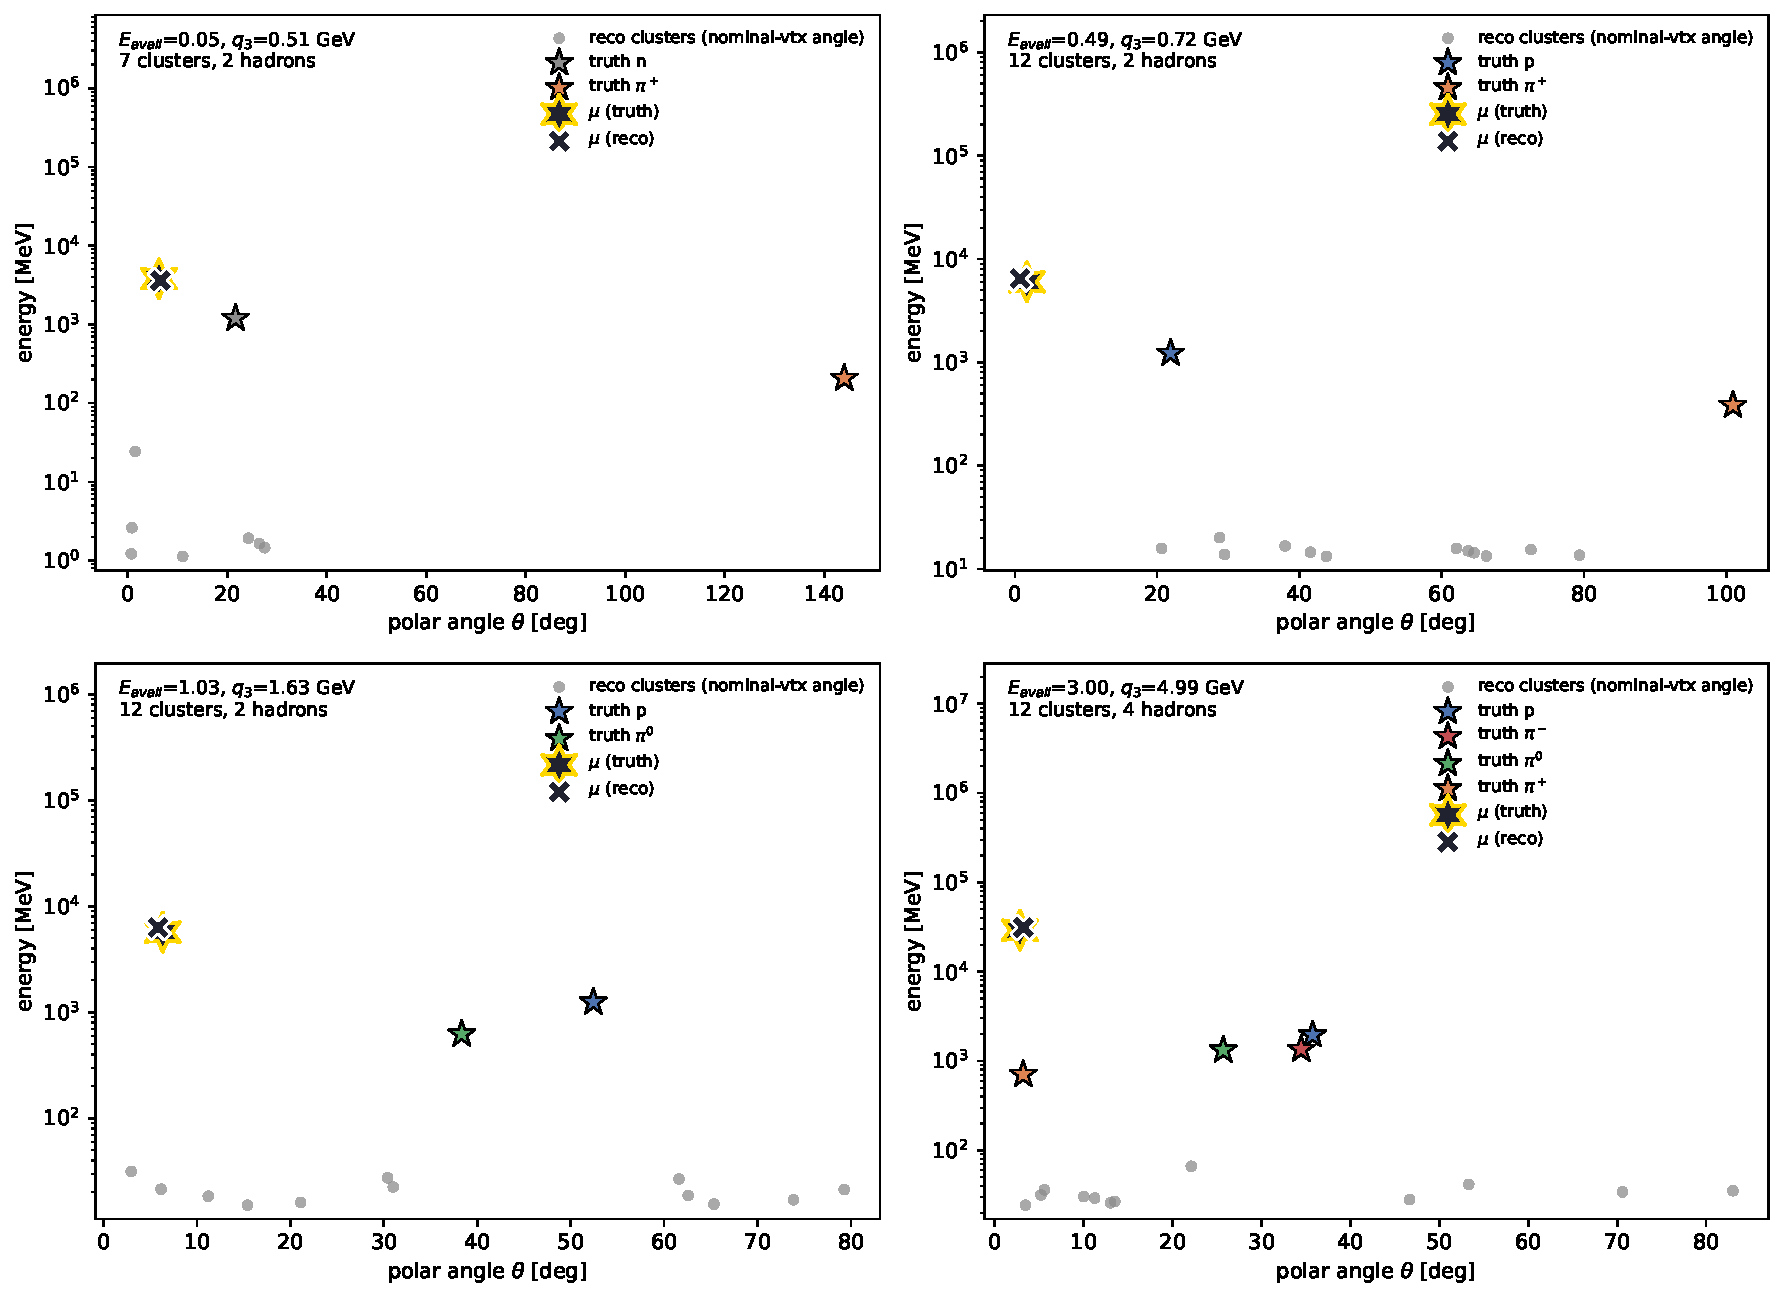
\includegraphics[width=0.98\textwidth]{pet_event_displays_energy_angle}
  \caption{Four representative PET events on a common energy--polar-angle
  plane. Gray points mark reconstructed recoil clusters, colored stars truth
  final-state hadrons. Reconstructed (X) and truth (six-point star) muons nearly
  overlap. Muon momentum and direction come from the MINERvA--MINOS track and
  are stored as event-level $(\pT,\pPar)$ scalars. The illustrative cluster
  angle uses a nominal upstream vertex: the current reco-cloud dump stores
  $[E_{\rm dep},\mathrm{pos}_{\rm
  view},z]$ without the reconstructed vertex. The common projection is only
  a visual comparison. PET consumes raw single-view clusters at reco level
  and hadron four-vectors at truth level; both recoil-only inputs omit the
  muon (Table~\ref{tab:pet-inputs}).}
  \label{fig:petdisplays}
\end{figure}

\begin{figure}[H]
  \centering
  % _withremnant shows the truth cloud inputs to PET (including GENIE nuclear-remnant
  % pseudo-particles), which produces the depleted k=1 bin.
  % _real is the physical-hadron-only version.
  %   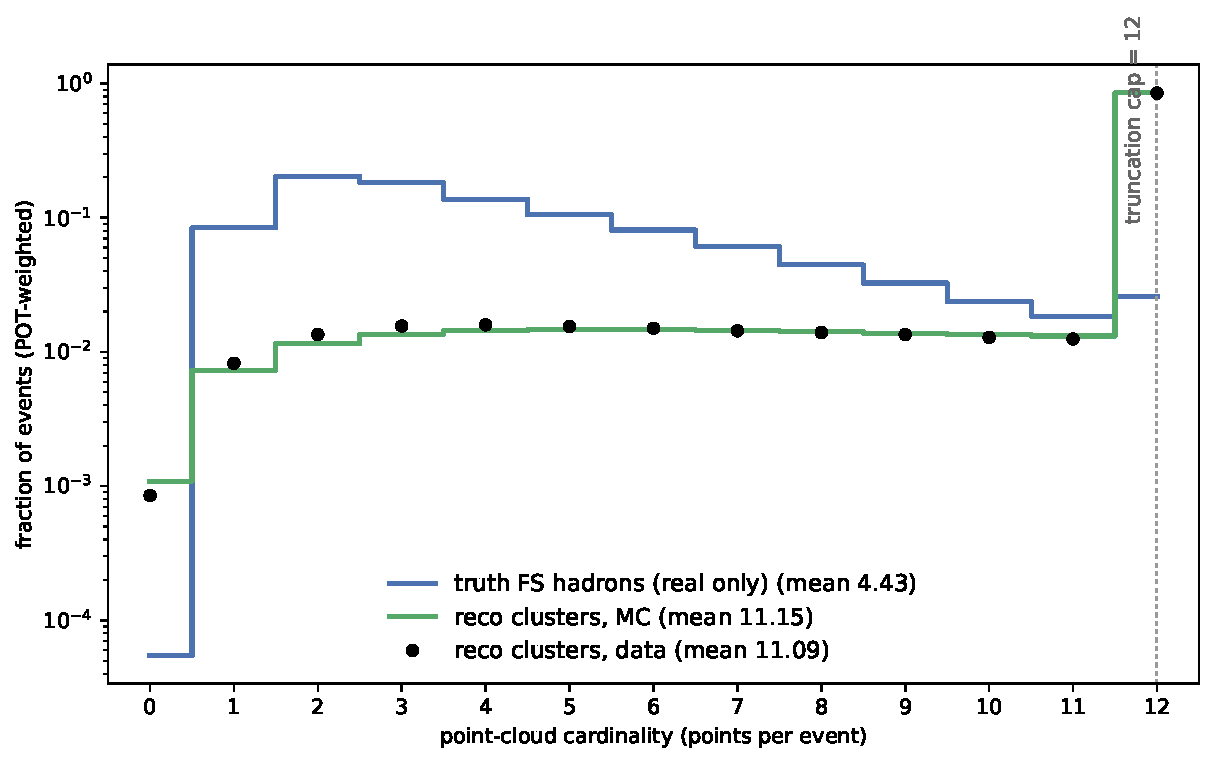
\includegraphics[width=0.72\textwidth]{pet_cardinality_real}
  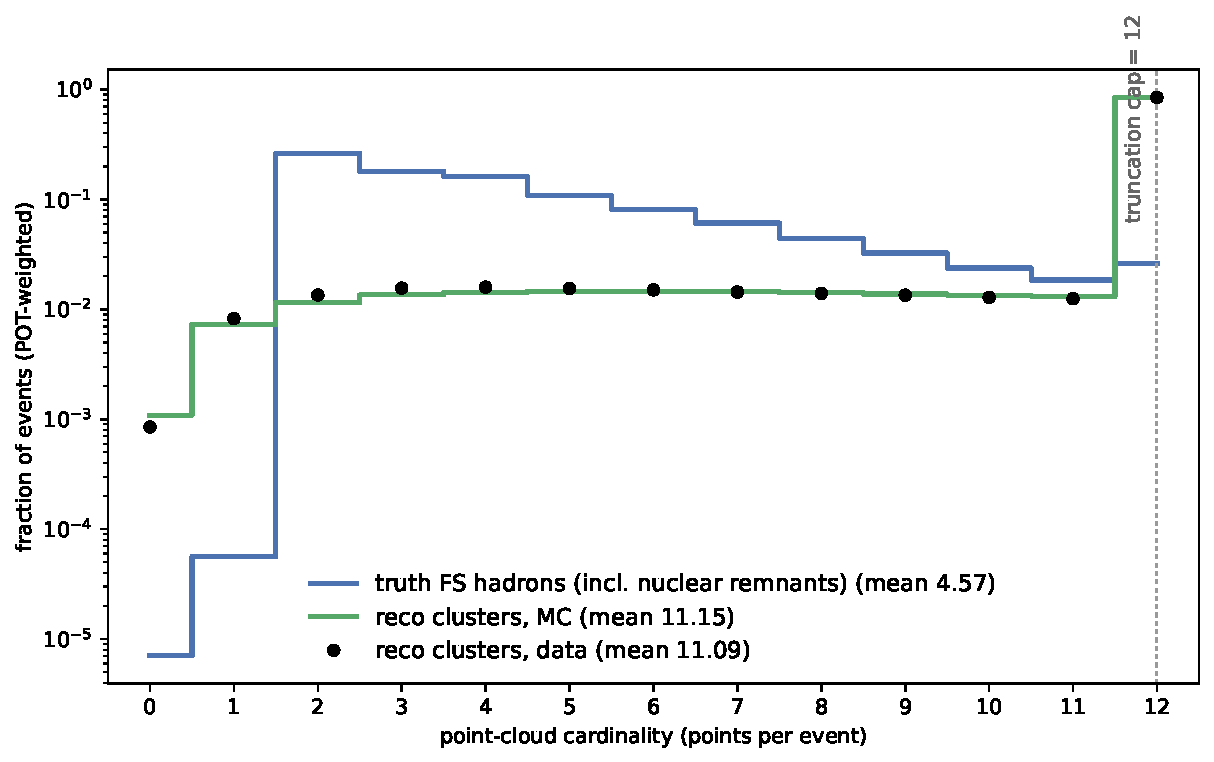
\includegraphics[width=0.72\textwidth]{pet_cardinality_withremnant}
  \caption{POT-weighted per-event point-cloud cardinality (constituent count)
  for truth final-state hadrons and reconstructed clusters in MC and data.
  Reco-cluster multiplicity greatly exceeds truth hadron multiplicity because
  a single hadron deposits
  energy in many detector clusters. Data and MC reco agree closely
  (means \num{11.09} vs.\ \num{11.15}). Retaining only the twelve highest-energy
  constituents makes reco distributions pile up at the cap. Truth clouds are
  sparser (mean \num{4.57}, including GENIE nuclear-remnant bookkeeping
  particles) and rarely reach it. The text explains the depleted $k=1$ truth
  bin and the truncation choice.}
  \label{fig:petcardinality}
\end{figure}

\paragraph{What comes out.}
\label{sec:pet-output-contract}
The classifier score is not the scientific result. PET probabilities, implemented through raw logits, are intermediate
density-ratio estimates; PET emits no binned network prediction. OmniFold converts the final
truth-step logit to an unbinned push weight for each simulated truth event,
$w_{\rm push}=\exp(\mathrm{logit})$. The cross section follows by weighting the
stored truth inventory, histogramming the requested observable, and applying
standard flux, target and bin-volume normalization~\cite{Andreassen:2019cjw}.
Any supported function of the stored truth record or retained truth cloud can
then be projected without retraining. Projection cannot create configurations
outside generator support, recover constituents above the cloud cap, or
convert recoil-only weights to full-event weights.

\subsection{Shape cross-check against the scalar result}
\label{sec:pet-shape}
The first use of the recoil representation is a shape comparison against the production
scalar unfold, which tests the classifier family and the engineered-scalar versus
recoil-cloud input choice together.
% Here \texttt{cluster\_pos} is the measured coordinate in one X/U/V scintillator view.
Area-normalized against the frozen 4D GBDT result, the PET unfold
reproduces the scalar shape to a median \SIrange{2.3}{3.9}{\percent} per bin
($\pT$~\SI{3.9}{\percent}, $\pPar$~\SI{2.4}{\percent}, $\Eavail$~\SI{2.6}{\percent},
$q_{3}$~\SI{2.3}{\percent}; Fig.~\ref{fig:petgbdt}).
The remainder of this section takes the same
representation from this shape check to an absolutely-normalized cross section.

\begin{figure}[H]
  \centering
  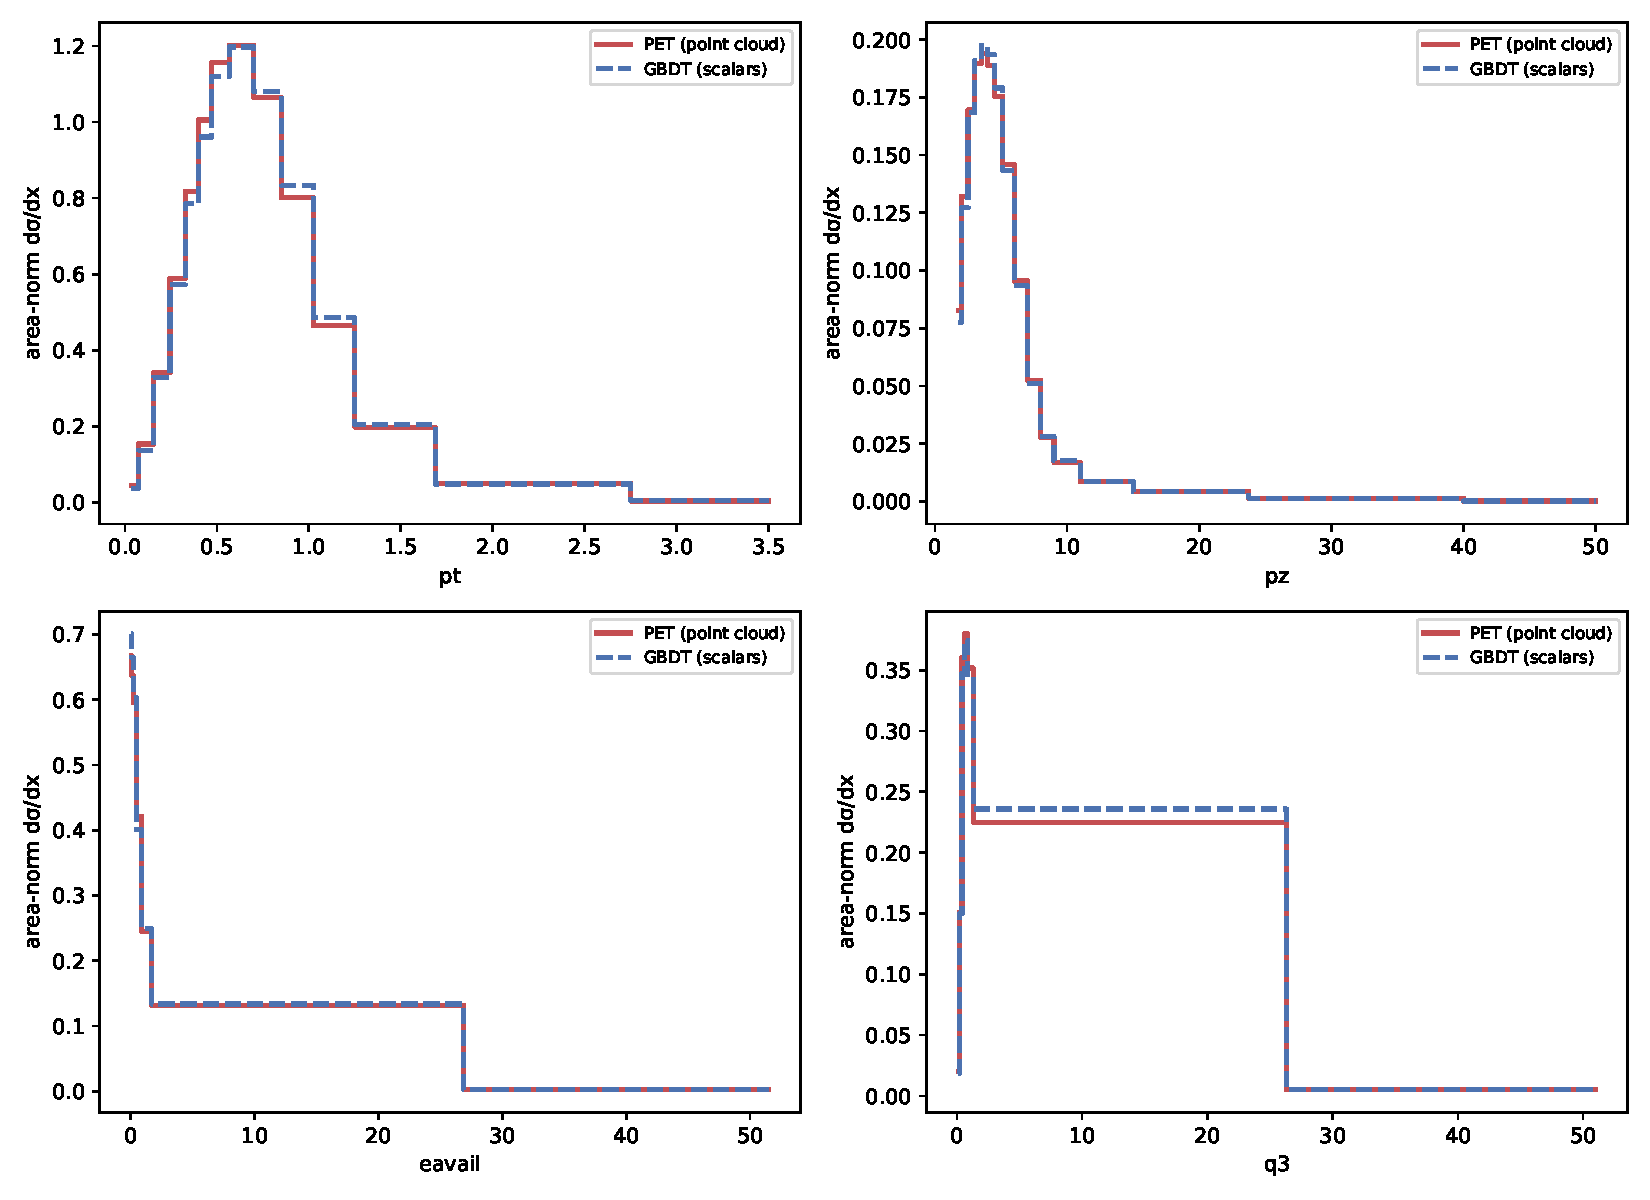
\includegraphics[width=0.85\textwidth]{pet_vs_gbdt}
  \caption{Area-normalized 4D unfolded shapes from the
    recoil-only PET point-cloud transformer (solid)
    and production scalar GBDT (dashed), projected onto each axis. Median
    per-bin shape differences are \SIrange{2.3}{3.9}{\percent}. The only visible
    deviation, in the wide $q_{3}$ catch bin, is a binning artifact: the bin
    collects a large, structured high-$q_{3}$ tail and does not indicate a
    genuine shape disagreement. This is a shape-only comparison (PET on a
    2M-event subsample), not an independent physics result.}
  \label{fig:petgbdt}
\end{figure}

\subsection{From shape check to absolute cross section}
\label{sec:pet-abs}
PET trains on a GPU with a 2M-event subsample (2 OmniFold iterations).
Its step-2 truth reweight is applied to the \emph{full} 32.8M-event generator
sample, binned on the 4D grid and passed through standard extraction. The
extraction uses the GBDT run's reweight-independent completeness and the same
flux/POT/nucleon constants (App.~\ref{app:provenance}, \texttt{pet-code}).
The absolute path had two checks:

\begin{enumerate}[itemsep=2pt]
  \item Pushed weights over all 32.8M generator events are finite, with mean
        $1.028$.
  \item Ordinary closure used MC-reco-as-pseudo-data at only two iterations.
        It is a legacy self-consistency diagnostic, not a current validation;
        no current closure level is quoted
        (App.~\ref{app:provenance}, \texttt{pet-closure-legacy}). Pseudo-data
        and prior share the same simulation, so this test cannot expose
        omitted muon dependence at fixed recoil.
\end{enumerate}

\paragraph{No current real-data PET--GBDT level of agreement is quoted.}
The historical real-data comparison used two-iteration training, preceded the 2026-08-01
full-event schema change and lacked background subtraction. It has not been
re-extracted under the pinned configuration. The legacy closure level and
higher-epoch retrain response are withdrawn on the same grounds
(App.~\ref{app:history}; App.~\ref{app:provenance}, \texttt{retracted-values}).

Ordinary closure alone cannot uniquely attribute a data-side gap to training
configuration. The recoil-only feature contract adds another difference:
at fixed recoil, the conditional muon distribution is inherited from the prior.
These structural limits survive the withdrawn numerical comparison.
The later simulation-only comparison in \S\ref{sec:pet-gbdt-paired}
does not revive it.

\subsection{Statistical and training diagnostics of the recoil-only estimator}
\label{sec:pet-syst}
PET statistical replicas independently Poisson-fluctuate data and MC, retrain
at a fixed estimator seed, and use the same coherent MC draw for final truth
binning and completeness.

The replicas and nominal use scalar GBDT's background-subtracted
five-dimensional measured target, unlike the legacy comparison in
\S\ref{sec:pet-abs}. Data align exactly event by event; MC arrays are
byte-identical to the full-cloud input. Ordering, event-alignment and
finite-output gates passed for the nominal extraction, an identical-seed
GPU-floor repeat, a 20-member coherent-Poisson retraining ensemble, and a
12-member crossed subsample/estimator-seed ensemble. GPU nondeterminism is
negligible relative to sampling and training variation. The recoil-only
statistical block measures diagnostic dispersion from 20 coherent replicas;
a 100-replica ensemble has not been run. It is not an independently verified
covariance or the statistical uncertainty of any PET result, and is not paired
with a PET central value. More replicas would sharpen dispersion estimates
without supplying coverage evidence.

\emph{This block is not the full-event} $C_{\rm stat}$ \emph{of
App.~\ref{app:cstatlimit}} (App.~\ref{app:provenance}, \texttt{cstat-family}).
The constructions and populations differ: 20 recoil-only replicas versus
50 full-event members, with two resampled inventories versus three.
Neither object's measurements, disclaimers or rulings transfer to the other.

No uncertainty is quoted from the historical recoil-PET assembly of vertical,
retraining, ML, statistical and detector blocks (App.~\ref{app:history}).
% Cut here (lane 3 §9.3 #2); the reasons survive at App. H (app:history-petbudget), the
% "no current level" statements at sec:pet-abs:
% adding the separate frozen-map
% and retraining covariances omits their cross term, and the detector block is
% CV-support-limited (App.~\ref{app:history}).  This section therefore
% retains the recoil-only central extraction and ordinary closure as historical
% method-development diagnostics.  It quotes neither a current PET--GBDT agreement
% level nor a current closure level, and no recoil-only covariance is paired with
% a PET central value.

\subsection{Truth-cloud projection within the recoil cross-check}
\label{sec:pet-projection}

Each recoil-only PET truth event carries the generator-level hadron cloud
(top-12-by-energy hadrons with PDG codes, built by
\texttt{CVUniverse::GetTruthFSHadrons})
% truth cloud branch: \texttt{part\_gen}
alongside its learned step-2 push weight. Re-binning these weighted events
projects any observable of the stored 4-vectors without retraining or
re-unfolding. We demonstrate this \emph{reweight-then-project} capability on
three observables computed post-hoc from the stored cloud: available energy
$\Eavail$ (the exact operational definition in
\S\ref{sec:eavail-definition}), hadronic-system invariant mass
$W_{\text{had}}=\sqrt{(\sum E)^2-|\sum\vec p|^2}$, and proton/charged-pion
multiplicities, while quantifying the cloud's two limitations.

\paragraph{Truncation is essentially lossless.}
Cloud-recomputed and dump-time $\Eavail$ use the same formula and inputs,
so their residual isolates truncation to the 12 highest-energy hadrons.
Over all \num{32.8}~million truth events (every event now carries a cloud, below),
the residual has median \SI{0}{MeV}, mean \SI{\pcEavailMean}{MeV}, and
\SI{\pcEavailWithin}{\percent} of events within \SI{10}{MeV}
(Fig.~\ref{fig:pcvalid}). The deficit occurs entirely in the
\SI{\pcSaturated}{\percent} of events saturating the 12-particle cap
(median deficit \SI{\pcSatDeficit}{MeV} there, exactly zero below it). Energy ranking
removes the lowest-energy stored final-state hadrons, giving a small,
one-sided, bounded effect. The 12-particle cap therefore does not limit $\Eavail$-scale
observables and does not need raising.

\paragraph{Coverage: closing the acceptance gap.}
The truth-only ``miss'' events appended for the unfold (\SI{\pcMiss}{\percent} of
the truth sample) carry a cloud: the truth final-state hadrons are carried through the
truth-denominator loop, filling the truth cloud for the appended miss
rows (the reco cloud correctly stays empty for a miss;
% branches: truth cloud \texttt{part\_gen}, reco cloud \texttt{part\_reco}
App.~\ref{app:history}). Coverage is complete:
\SI{\pcHasCloud}{\percent} of truth events carry clouds, leaving only
\pcEmptyCloud{} residual empties out of \num{32.8}~million. Cloud-recomputed
$d\sigma/d\Eavail$ reproduces the full unfold to
$\lesssim\SI{\pcCloudFull}{\percent}$ in every $\Eavail$ bin; the projection
is no longer acceptance-limited.

Three $\Eavail$ projections overlay in the centre panel of
Fig.~\ref{fig:pcxsec}: push-weighted cloud and stored $\Eavail$ on the
has-cloud subset, and stored $\Eavail$ over the full unfold. Their largest
relative per-bin spread is
\SI{\pcCloudFull}{\percent}. No reco-efficiency division is applied because
unfolded counts are already acceptance-corrected
(App.~\ref{app:history}; App.~\ref{app:provenance}, \texttt{pet-projection-figure}).
% Summary keys: \texttt{pet\_cloud\_hascloud}, \texttt{pet\_stored\_hascloud}, \texttt{pet\_stored\_full}.

\paragraph{Exploratory projection yields new hadronic diagnostics.}
$W_{\text{had}}$ measures the true hadron-system invariant mass. The
leptonic ``experimenter's'' $W$ stored at dump time is reconstructed from muon kinematics assuming
a single struck nucleon at rest; $W_{\text{had}}$ is not its lossy copy.
Their median difference is \SI{\pcWoffset}{GeV}. The 2D correlation
(Fig.~\ref{fig:pcxsec}, left) has a sharp locus at
$W_{\text{had}}\approx\SI{0.94}{GeV}$ for single-baryon final states: their
hadronic mass equals the nucleon rest mass irrespective of leptonic $W$.
Fermi-smeared diagonal bands rise by $\sim$one nucleon mass per extra
final-state baryon (multi-nucleon knockout, 2p2h). The projection thus supplies
a physically interpretable hadron-cloud diagnostic from the recoil-only unfold.

\begin{figure}[H]
  \centering
  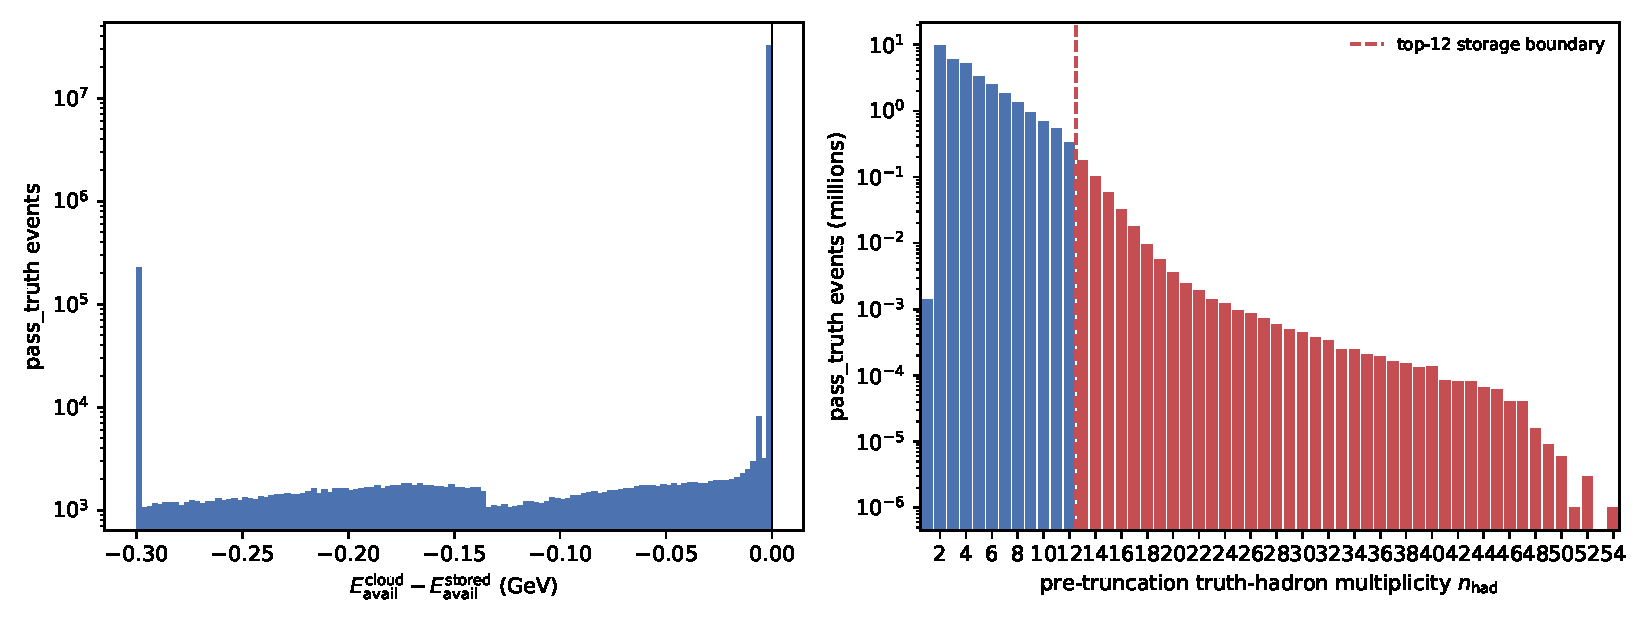
\includegraphics[width=0.90\textwidth]{pet_cloud_projection_validation}
  \caption{Cloud-recomputed $\Eavail$ minus its dump-time value over all
  \num{32.8}~million truth events. The residual is zero to
  \SI{\pcEavailWithin}{\percent} within \SI{10}{MeV}; its small negative tail
  occurs only in the \SI{\pcSaturated}{\percent} reaching the 12-hadron cap.
  Right: ordinary event counts versus pre-truncation multiplicity from the
  variable-length ROOT branch. Multiplicities 1--12 are exact; sparse tails
  are grouped into labeled 13--14, 15--17, 18--24, and $\geq25$ categories.
  The dashed boundary separates fully stored events from categories retaining
  only the 12 highest-energy hadrons. Cap-reaching events have median
  $\Eavail$ deficit \SI{\pcSatDeficit}{MeV}. Keeping the 12 highest-energy hadrons is therefore
  essentially lossless for $\Eavail$-scale observables.}
  \label{fig:pcvalid}
\end{figure}

\begin{figure}[H]
  \centering
  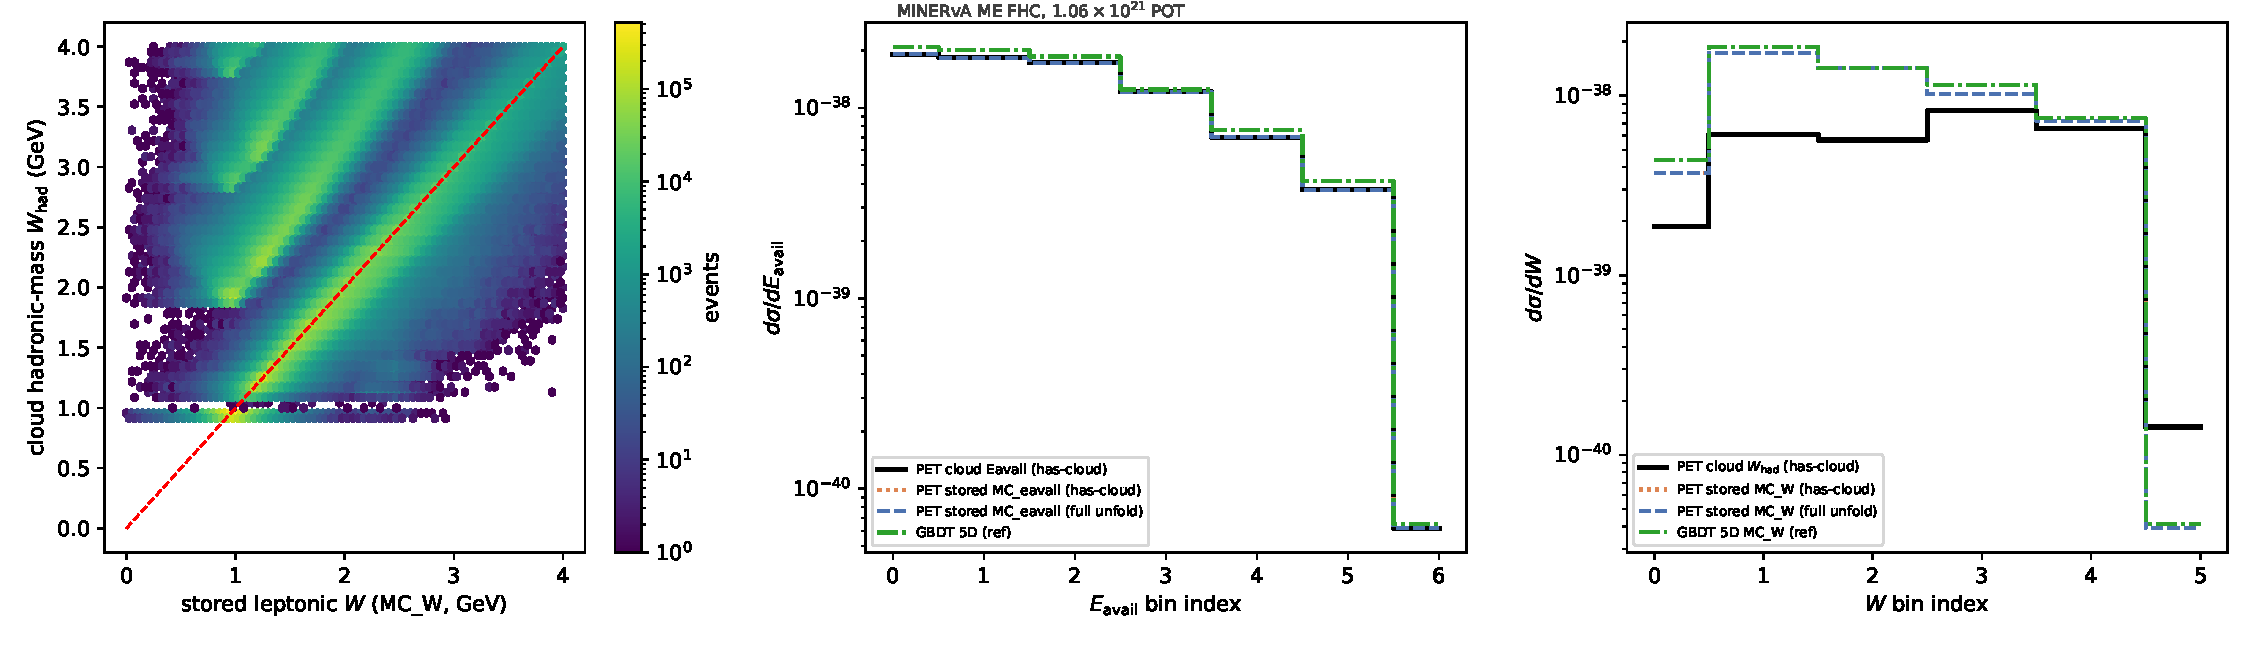
\includegraphics[width=0.98\textwidth]{pet_cloud_projection_xsec}
  \caption{Exploratory recoil-only reweight-then-project demonstration.
  \emph{Left:} hadronic-system invariant mass $W_{\text{had}}$ versus stored
  leptonic $W$. Their definitions differ (median \SI{\pcWoffset}{GeV}); the
  QE locus is at \SI{0.94}{GeV}, with multi-baryon bands above $y=x$.
  \emph{Center:} projected $d\sigma/d\Eavail$. Push-weighted cloud $\Eavail$,
  stored $\Eavail$ on the has-cloud subset, and stored $\Eavail$ over the full
  unfold agree to $\lesssim\SI{\pcCloudFull}{\percent}$ per bin because
  essentially every truth event carries a cloud after the coverage fix.
  The different GBDT 5D estimator is not expected to coincide.
  \emph{Right:} projected $d\sigma/d W_{\text{had}}$, whose shape differs
  from the leptonic-$W$ reference as expected.}
  \label{fig:pcxsec}
\end{figure}

\paragraph{The projection and extrapolation limits.}
\label{sec:pet-projection-next}
Reweighting can only redistribute weight among truth configurations the
generator already produced; it cannot populate phase space the prior never
sampled --- the same extrapolation limit flagged for the extended-fiducial
study (\S\ref{sec:fps}). Hadron-cloud diagnostics can be projected within that
stored spectrum. They cannot convert recoil-derived weights to full-event
weights or remove the prior conditional for omitted muon information.
The stored recoil-only result cannot acquire the later full-event estimator's
muon dependence: those are separate estimators with the
distinct interfaces in Table~\ref{tab:pet-inputs}.
Re-projection also cannot recover rare very-high-multiplicity constituents
above the 12-particle cap, which the validation finds unnecessary at
$\Eavail$ scale. Details and reproduction are in App.~\ref{app:provenance}
(\texttt{pet-projection-figure}).

\subsection{Extended population and the full-event candidate}
\label{sec:pet-full-event-status}

\paragraph{Recoil-PET feasibility study on the extended population.}
\label{sec:fps-pet}
The feasibility study on the enlarged population and reporting grid of
\S\ref{sec:fps} remained recoil-only. Step~1 used non-muon reco clusters;
step~2 used truth hadrons with the muon removed. Muon coordinates defined
and binned the extension but were absent from classifier inputs. The
populated-bin counts, prior-transfer envelope and retraining floor are
recoil-estimator feasibility diagnostics, not a final full-event measurement;
they are not used to argue that low-efficiency cells are data-constrained.

A full-event estimator on this population would carry the requirements set out
above, and additionally consume the canonical extended-fiducial event loops
and $15\times19$ muon grid while preserving the enlarged truth denominator, native
misses and unchanged reconstructed selection. Additional features can use more observed
information, but cannot create detector information in zero-efficiency cells.

\paragraph{Full-event artifacts and present boundary.}
Within its recoil-only contract, the study demonstrates end-to-end paired reco/truth cloud
construction, GPU training, full-sample reweighting, absolute cross-section
extraction, coherent bootstrap replicas and the response studies above.
It does not establish simultaneous muon-plus-hadron unfolding, because the muon
was absent from classifier inputs.

Later full-event extended-FPS work has a nominal artifact and a 50-member
$C_{\rm stat}$ artifact. The latter has one builder, is not independently
verified or adopted, and was declined for pairing with the nominal
(status paragraph above).
% Joseph declined pairing it with the nominal on 2026-08-20.
% Cut as a restatement of the status paragraph (lane 5 R8): "and requires
% estimator-equivalence plus coverage evidence before reconsideration" and "and no PET
% covariance is adopted as a publication uncertainty". Gate 6 and the five receipt
% prohibitions moved to App. E (pet-gate6).
The ruling neither invalidates the measured dispersion nor establishes a
mechanism. A spatially coherent anomaly remains with unvalidated coverage.
No $C_{\rm ML}$ or full PET total covariance exists, and starting a PET
ML-variance component is not authorized
(App.~\ref{app:provenance}, \texttt{pet-gate6}). App.~\ref{app:cstatlimit}
records the construction and limitations. None of these artifacts changes PET's diagnostic and method-development status.

\subsection{Completed simulation studies of PET design}
\label{sec:pet-campaigns}

The improvement and final-design studies tested whether better point estimates
could be combined with a calibrated uncertainty procedure. They improved
recovery substantially, but the terminal selection outcome is
\texttt{NO\_ELIGIBLE\_DESIGN}: no design or default was selected.
All results below concern signal-only simulation and method development,
not a real-data cross section or a publication uncertainty product
\cite{PETImprovement2026,PETFinalDesign2026}.

For unit-normalized histograms, recovery is
\begin{equation}
 R=1-\frac{\sum_b|u_b-t_b|}{\sum_b|p_b-t_b|},
 \label{eq:pet-campaign-recovery}
\end{equation}
where $u$, $t$ and $p$ are the unfolded, pseudodata-truth and prior
distributions on the stated reporting histogram. Thus $R=1$ is exact
recovery, $R=0$ retains the prior's discrepancy, and $R<0$ moves farther
from the target. A nearly unchanged marginal makes the denominator small;
joint hadron-content histograms and absolute residuals are needed in such
cases. This metric differs from the historical cellwise recovery proxy in
\S\ref{sec:gbdt-model-dependence}.

\paragraph{Improvement study: recovery gains did not qualify a design.}
Development, pilot, final and stress samples had separate roles. On twelve
fresh final draws, the historical PET control at three iterations recovered
$R=0.316$ of the seven-bin $\Eavail$ tilt. The frozen interventions at
$K^*=10$ gave the results in Table~\ref{tab:pet-improvement}.

\begin{table}[htbp]
\centering
\small
\begin{tabular}{@{}lrr@{}}
\toprule
Frozen intervention & Mean $R$ & One-sided 95\% lower bound \\
\midrule
A: iterations alone & 0.505 & 0.490 \\
B: reco summaries and one-hot truth PDG & 0.569 & 0.555 \\
C: efficiency-corrected truth step & 0.786 & 0.763 \\
\bottomrule
\end{tabular}
\caption{Improvement study at its declared ten-iteration operating point,
twelve final draws per configuration. B retains the carry-misses rule;
C trains the truth-step ratio on selected events and extrapolates it to
missed events. The unchanged aggregate adequacy floor is 0.556, with
additional regional mean requirements. B passes the point rule but its
lower bound is below the floor; A fails and C clears it. B versus A combines
two input changes and does not isolate the reco summaries.}
\label{tab:pet-improvement}
\end{table}

The 36 final and 36 stress runs completed. Coverage was not run: no frozen
candidate at $K^*=10$ met both adequacy and the stress requirement.
B moved away under neutron-content reweighting, and C under proton- and
neutron-content reweighting, despite these distortions being distinguishable
at reconstruction level. There were only two stress draws per case.
C at three iterations met the mean adequacy rule and had no moves-away
stress cell, but its lower bound was below the floor and that iteration was
not the frozen coverage point. It was not retrospectively promoted.
The combined detector-scale-plus-tilt case had no matching identifiability
test or unscaled control on the same draws; its recovery does not isolate
the response effect. The review left the PET failure mechanism unestablished.
Subsequent development showed that the predecessor's C neutron case barely
changed the scored marginal, whereas B made a genuine wrong-direction
push. These diagnostics motivated the next study without changing the
predecessor's frozen verdict.

\paragraph{Final design: representation, training and seed reproducibility.}
The next study used fixed development, final and sealed reserve banks.
Each unfolding had about 600,000 prior events and 600,000 pseudodata events;
final inference is conditional on those banks. Detector energy summaries
helped recover information omitted by the stored top-12-cluster cloud.
Categorical truth PDG encoding, a constant per-iteration learning rate and
longer truth-step training completed the hybrid designs. In development,
extending the truth step to 24 epochs reduced the fixed-event seed SD of
the primary recovery to 0.037 and 0.043, below the 0.05 limit. These are
seed-reproducibility measurements, not uncertainty coverage.

The frozen finalists were compact H2S1T24 at five iterations and larger
L128S1T24 at four, with approximately 47,000 and 970,000 detector-step
parameters. Pretrained PET2 improved on its scratch counterpart, but no
tested PET2 design passed all development screens: the stable annealed
variant failed the proton-topology screen. This is a result for the tested
recipes, not a general rejection of pretraining.

On 60 final-bank tilt draws, H2S1T24 and L128S1T24 reached
$R=0.895$ and $0.863$, respectively, against the historical PET control's
$0.306$. H2S1T24 passed the frozen accuracy, robustness and stability rules.
L128S1T24 failed B2, the neutron-down test on the nearly unchanged
$\Eavail$ marginal: mean residual minus
injected $L_1$ was $0.0122$, above $0.010$, versus H2S1T24's $0.0097$.
Both 95\% intervals cross the threshold, so the frozen point rule decides
eligibility but the statistical comparison establishes neither a robustness
ranking nor equivalence. The frozen B1 independence-based bound passes;
within-draw dependence prevents establishing its intended per-unit failure
probability bound. Nor does it show that the per-unit failure probability exceeds 0.10.
The compact design was not cheaper at the declared packing, so the
cost-based preference for it did not apply.

\paragraph{Coverage fails, with opposite behavior across acceptance regions.}
The H2S1T24 interval procedure uses six independent Poisson-bootstrap
members, each with its own training seeds. Its estimate is their mean
normalized histogram; intervals are
$\bar u\pm t_5 s\sqrt{1+1/6}$ at the stated confidence level, where $s$
is the member SD. On 120 final-bank development-tilt draws (720 unfoldings),
the results are those of Table~\ref{tab:pet-final-coverage}.

\begin{table}[htbp]
\centering
\small
\begin{tabular}{@{}lrr@{}}
\toprule
Scored region & Nominal 68\% coverage & Nominal 95\% coverage \\
\midrule
Aggregate $\Eavail$ & 0.896 & 0.990 \\
Low acceptance & 0.257 & 0.789 \\
Moderate acceptance & 0.701 & 0.964 \\
Good acceptance & 0.929 & 0.998 \\
\bottomrule
\end{tabular}
\caption{H2S1T24 K5 six-member interval coverage against each draw's own
pseudodata truth. Aggregate intervals over-cover: C1 fails decisively at
68\% (lower bound 0.858, ceiling 0.80). C4 also fails: mean 95\% half-widths
in six of seven bins are 1.32--1.72 times the allowed limit. Low acceptance
under-covers; no frozen rule gates that region (C3 covers only the moderate
and good regions). C2 and C3 pass.}
\label{tab:pet-final-coverage}
\end{table}

Each entry pools checks of bin values over the 120 draws: it counts intervals
containing their target, not events classified correctly. It is not the
probability that every bin is covered simultaneously. The draw-specific truth
target differs from the fixed unfluctuated population used in the 2D test
(\S\ref{sec:coverage}).

The same over- and under-coverage pattern survives comparison with the
final-bank population target. Its mechanism is not established; it is not
uniform conservatism. The proton-topology coverage stage C5 was skipped
after the decisive failure, and L128S1T24 coverage was never measured.
The terminal outcome remains \texttt{NO\_ELIGIBLE\_DESIGN}: H2S1T24 fails
interval calibration and L128S1T24 fails B2 by the frozen point rule (statistically
unresolved). Neither failure proves that the
point estimator is unusable. No repair or reserve-bank revalidation forms
part of these completed results.

\paragraph{Computational cost and what it establishes.}
Table~\ref{tab:pet-cost} separates measured study resources from projections
to real-data scale~\cite{PETFinalDesign2026,PETGBDT2026}.
The comparison buys evidence about recovery on the specified simulation
banks, not a calibrated uncertainty product. CPU core-hours and A100-hours
are different resources, so these values do not establish a
hardware-normalized speedup or a universal architecture ranking.

\begin{table}[htbp]
\centering\footnotesize
\begin{tabular}{@{}p{0.24\textwidth}p{0.30\textwidth}p{0.37\textwidth}@{}}
\toprule
Configuration & Population and repetitions & Resource use and status \\
\midrule
Compact PET H2S1T24, $K=5$ & About 600k prior and 600k pseudo-data events; 352 final-bank units & Measured median 1.768 A100-h per unfold; no eligible interval procedure \\
\addlinespace
Larger PET L128S1T24, $K=4$ & Same scale and 352 units & Measured median 1.517 A100-h per unfold; fails a frozen point rule, coverage unmeasured \\
\addlinespace
Paired scalar GBDT, $K=1$--10 ($K=7$ primary) & Same events; 352 tasks, control and retries & Measured 5.306 charged CPU core-h for the fitting campaign (4.422 process CPU-h); no uncertainty comparison \\
\addlinespace
PET at real-data scale & 2M-event prior; full selected data and background target & Forecast 7.3 / 7.1 A100-h per unfold (compact / larger), with factor-two ranges \\
\addlinespace
PET with full MC inventory & 49.15M-event prior; same real-data target & Forecast 136 / 119 A100-h per unfold, with factor-two ranges; not trained at this scale \\
\bottomrule
\end{tabular}
\caption{Measured PET costs use two unfoldings packed per A100. Forecasts scale
the measured training rates and retain each finalist's iteration count;
they are not observed production costs. The compact finalist was not cheaper
at its chosen operating point. GBDT cost is a campaign total, not a per-unfold
time.}
\label{tab:pet-cost}
\end{table}

\subsection{Exploratory PET--GBDT comparison on the same events}
\label{sec:pet-gbdt-paired}

The later comparison reused both finalists' point estimates and fitted a
scalar HistGradientBoosting OmniFold to the identical 352 final-bank units
per finalist, with the same events, weights, distortions, targets and scorer
\cite{PETGBDT2026}. Its efficiency-corrected miss treatment matches PET's;
detector inputs are muon kinematics, reconstructed $\Eavail$ and $q_3$,
stored-cluster energy sum and count. Truth inputs include four scalar
kinematics and species counts over the stored 12-token cloud, not full
particle multiplicities. The primary GBDT iteration, $k=7$, was chosen on
development data before final-bank use. This is a specific comparator,
distinct from the production scalar-5D LightGBM synthesis in
\S\ref{sec:gbdt-model-dependence}.

PET recovers both $\Eavail$ tilts better than this GBDT
(Fig.~\ref{fig:pet-gbdt-paired}). On the development tilt, paired gains in
$R$ are $+0.102$ [0.084, 0.119] for H2S1T24 and $+0.070$ [0.051, 0.089]
for L128S1T24 over 60 draws. Summed per-bin mean squared residuals are
$(3.33,5.26,9.78)\times10^{-4}$ for H2S1T24, L128S1T24 and GBDT.
Residuals compare each estimate to its own draw's target; their spread is
not unconditional estimator variance. On the proton-topology endpoint,
H2S1T24's gain at GBDT $k=7$ is $+0.055$ [0.035, 0.075], but at
$k=10$ it is $+0.009$ [$-0.012$, 0.030]; L128S1T24 is level at $k=7$
($+0.012$ [$-0.007$, 0.031]) and below the GBDT at $k=10$ ($-0.034$
[$-0.054$, $-0.015$]). The $\Eavail\times q_3$
endpoint does not resolve a difference.

\begin{figure}[htbp]
\centering
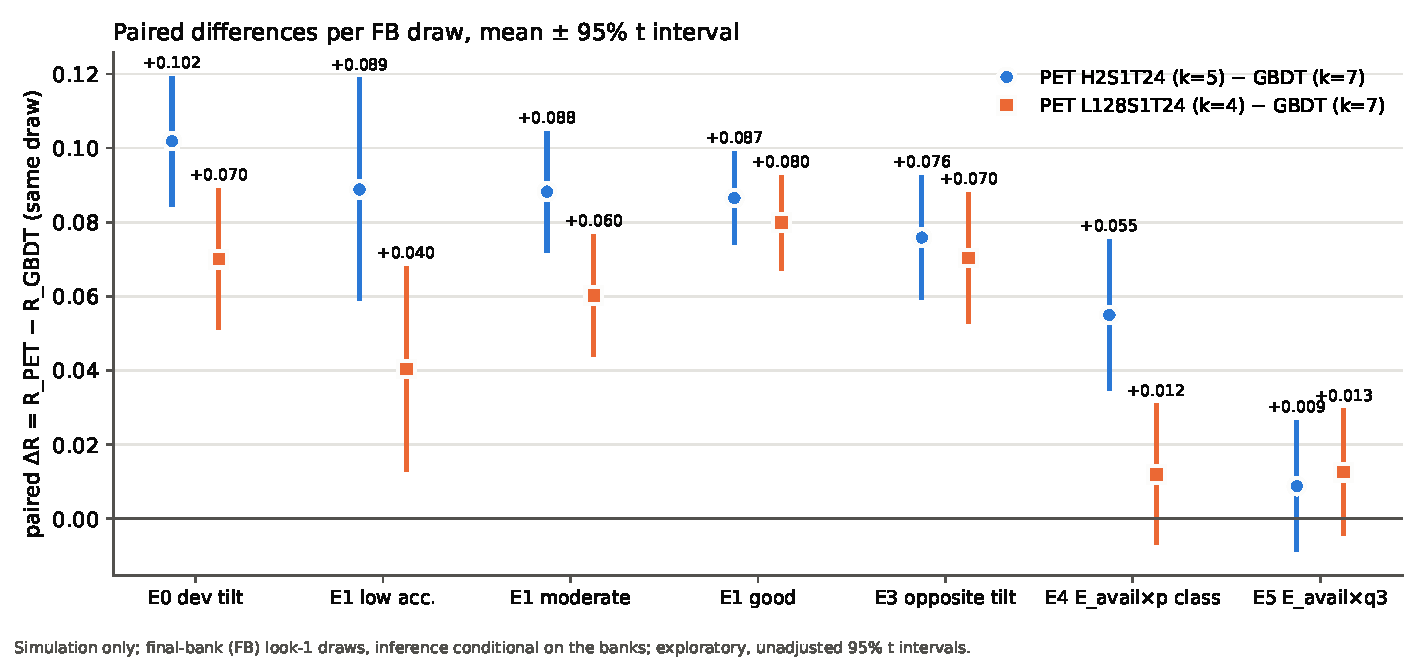
\includegraphics[width=\linewidth]{pet_gbdt_paired_differences.pdf}
\caption{Existing exact-paired comparison of the PET finalists with GBDT
at its development-chosen $k=7$. Positive differences favor PET.
E0 and E3 are the two $\Eavail$ tilts (60 draws); E1 subdivides E0 by
acceptance; E4 is $\Eavail\times$ proton class and E5 is
$\Eavail\times q_3$ (40 draws). Bars are unadjusted two-sided 95\%
Student-$t$ intervals, conditional on the frozen banks. Exploratory point
estimates only: no uncertainty comparison or finalist ranking follows.}
\label{fig:pet-gbdt-paired}
\end{figure}

The broader distortion library reverses some of this ordering
(Fig.~\ref{fig:pet-gbdt-library}). GBDT is better on all three tested
generator-model reweightings (NuWro, NuWro$'$ and GiBUU) by 0.12--0.25 in
$R$, and on the narrow energy bump. These are fixed-response simulation
reweightings, not independent detector simulations or real-data comparisons.
PET leads on several species distortions. Its raw muon-scale result largely
includes its underlying tilt gain: the response-specific paired contrast
is only $+0.016$ [$-0.005$, 0.037] for H2S1T24 and $+0.028$
[0.013, 0.043] for L128S1T24. Signed response contrasts alone are not
robustness rankings.

\begin{figure}[H]
\centering
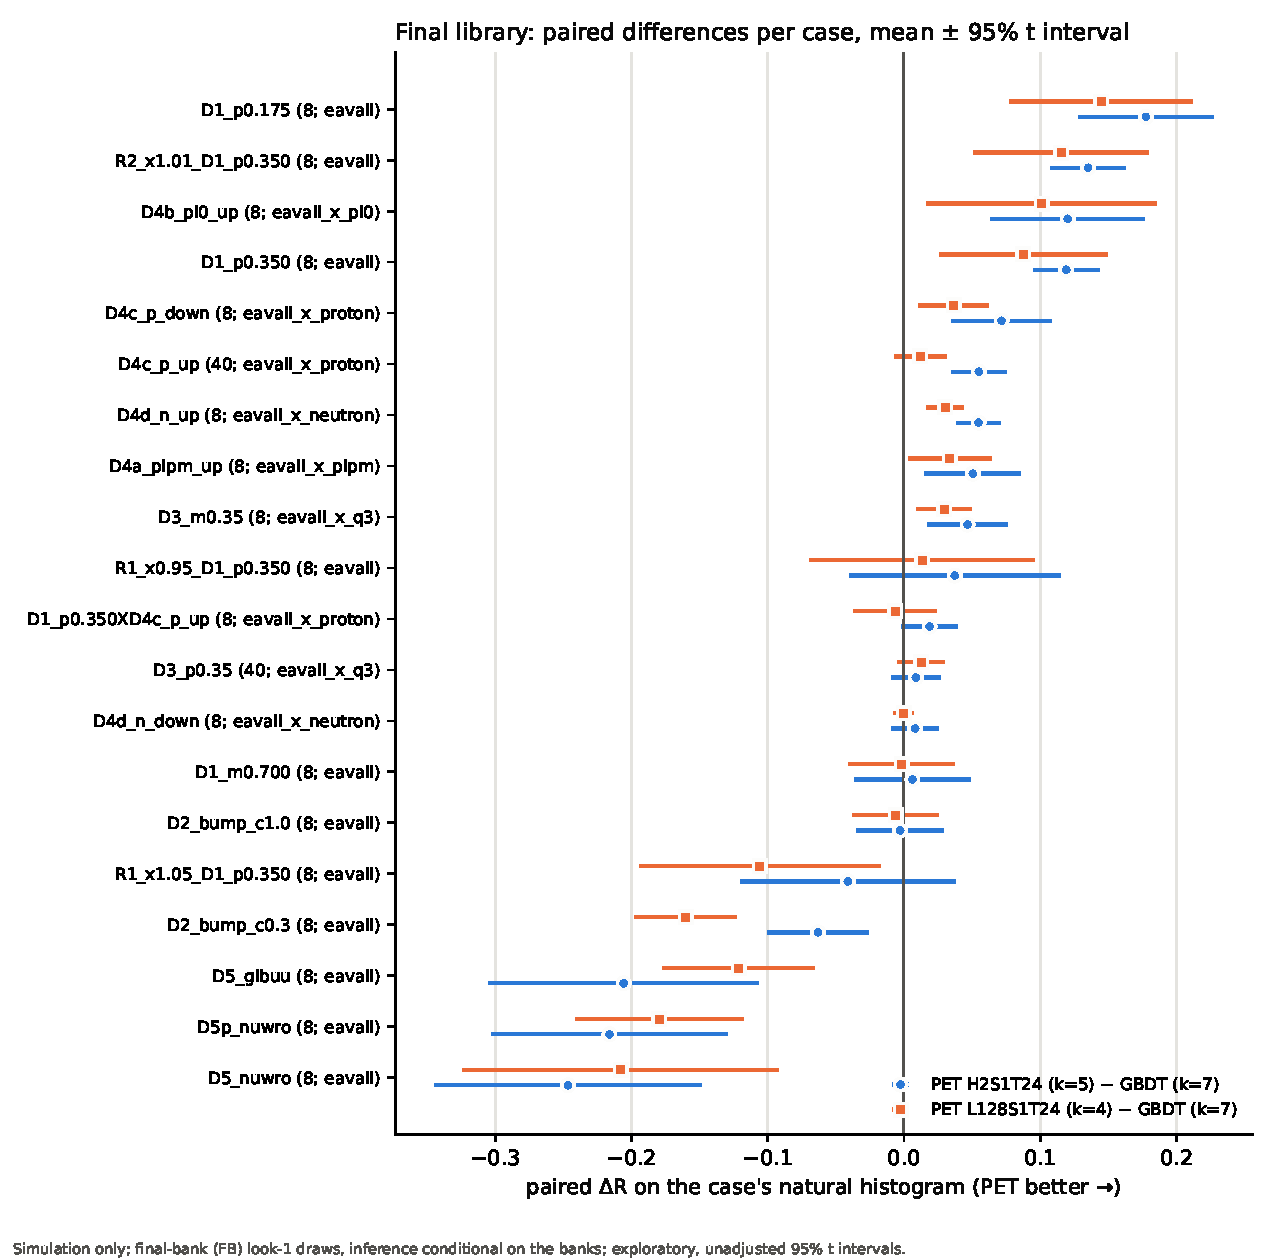
\includegraphics[width=0.94\linewidth]{pet_gbdt_library_paired.pdf}
\caption{Paired recovery differences across the existing distortion library,
GBDT at $k=7$. Each case uses its natural histogram; most have eight
draws, with D4c proton-up and D3 $+0.35$ ($\Eavail\times q_3$) using 40.
Intervals are unadjusted 95\% Student-$t$ intervals conditional on the
banks. The response-plus-tilt rows include the tilt contribution and do
not isolate detector-response sensitivity. The generator rows show that
PET's tilt advantage does not extend to every tested departure.}
\label{fig:pet-gbdt-library}
\end{figure}

All contrasts are exploratory: the PET final-bank results had already been
inspected, intervals are not adjusted for multiple comparisons, and inference
conditions on the finite banks at study scale (about 600,000 pseudodata
events per unfolding). On the two matched development draws (descriptive),
binned iterative Bayesian unfolding and AUSSIE with kinematic truth inputs
match or beat PET on the one-dimensional tilt but fail on hadron-content or
generator cases; the observed lead is over this HGB OmniFold, not scalar
unfolding in general. There is no GBDT interval procedure in this comparison,
and the measured PET procedure failed calibration. Thus no uncertainty
comparison, universal method ordering, finalist ranking or adoption follows.
The completed comparison leaves \texttt{NO\_ELIGIBLE\_DESIGN} unchanged.

The improvement and final-design numerical conclusions have the committed
independent checks recorded with their reports. The paired comparison's
numbers also reproduce independently; its post-second-review wording and
prospective design repairs were not re-reviewed. These distinctions do not
upgrade any result to publication uncertainty status. Ledger entries
VL164--VL168 record the final-design and comparison results; the cited
reports route the frozen decisions and closed review dispositions.


\subsection{Related representations and estimator-design outlook}
\label{sec:pet-gregor}
Gregor Krzmanc's \texttt{minerva-ml} uses the same broad MINERvA ME~FHC
simulation for supervised available-energy regression and charged-current-pion
classification with an OmniLearned/PET2 backbone~\cite{Krzmanc:2026transfer}.
At the pinned commit, typed muon, photon, prong and calorimeter-blob tokens
use collider-style $(\eta,\phi,\log p_T,\log E)$ coordinates, learned type
embeddings, $dE/dx$, position and timing. Prongs or blobs exceeding their
separate caps become aggregate overflow tokens.\footnote{Implementation comparison:
\href{https://github.com/gregorkrz/minerva-ml/blob/af5d92ed2b3b448a09b6b7cf6b4f179e5757b4ed/DATASET.md}{\texttt{minerva-ml DATASET.md}}
and
\href{https://github.com/gregorkrz/minerva-ml/blob/af5d92ed2b3b448a09b6b7cf6b4f179e5757b4ed/MODELS.md}{\texttt{MODELS.md}},
commit \texttt{af5d92ed}.}
Our reco leg uses generic detector-geometry calorimeter clusters without
reconstructed-object type embeddings and discards tokens beyond the common
top-12-by-energy cap. Our task estimates OmniFold density ratios against real
data with explicit backgrounds and native misses, rather than supervised
regression or classification on simulation. Typed reconstructed objects and
aggregate overflow tokens remain prospective representation improvements;
the present estimator uses neither.

\paragraph{Ensembling as an estimator-design choice.}
Neural likelihood-ratio studies find that Step~1 model averaging before
pushing weights to Step~2 can improve unfolding bias and variance
\cite{ToralesAcosta:2025stabilizing}. Averaging within iterations and averaging
final weights define different estimators. Future comparisons must specify
what is averaged, where in the iteration, and the nominal/replica pairing.
The same study finds that pretraining can reduce
variance while increasing bias, so seed dispersion alone is insufficient to
rank designs. Closure bias and uncertainty calibration must also be assessed.
These are method-development directions, not explanations of the existing
full-event anomaly, evidence for its declined pairing, or an adopted PET
uncertainty construction.


\section*{Acknowledgments}
This
analysis was carried out on the Perlmutter system at the National Energy
Research Scientific Computing Center (NERSC), a U.S.\ Department of Energy
Office of Science User Facility, under project m3246. It builds on the MINERvA
Analysis Toolkit (MAT) and the MINERvA-101 cross-section framework, and we thank
their authors. We are grateful to the MINERvA Collaboration for the public release
of the medium-energy CC-inclusive data product on which the reproduction rests.

We thank Callum Wilkinson for connecting us with this dataset and for many helpful discussions.

% The analysis note's statement, verbatim (main_note.tex acknowledgments).
The analysis code, statistical procedures, computing campaigns, independent
recomputations and reviews, figures, and manuscript drafts were produced with
substantial assistance from AI language-model tools, used through the Claude
Code and OpenAI Codex command-line agents: Anthropic Claude (Opus 4.7, 4.8, 5,
and 5.5; Fable 5 and 5.1) and OpenAI GPT models (GPT-5.5, GPT-5.6 Sol and Luna,
GPT-6 Astra, and GPT-6.1), including those used for independent review. The
authors directed this work through written specifications fixed before each
study. Results were accepted only after verification against committed
evidence: predeclared criteria, independent recomputation by separately written
code (for example, the joint-test evaluation and the lost-seed recovery), and
independent read-only reviews. AI tools were also used for methodological
discussion. The figures were drawn by plotting code
from the analysis outputs; no image was generated or edited by a generative-AI
image tool. AI tools are not authors. The authors take responsibility for the
content.

\appendix
% Moved verbatim from app_statmethods.tex (its last subsection) on 2026-10-11, so that the PET statistical method has its own appendix; labels unchanged. Moved with sec_pet.tex to the companion PET note (pet_note.tex) on 2026-10-12.
\section{The full-event $C_{\rm stat}$ construction: what it is, and what it is not}
\label{app:cstatlimit}

The published uncertainty is constructed in \notesec{Uncertainty quantification: constructing the covariance blocks}, with adopted five-axis covariance identified in \notesec{The adopted five-axis covariance and its $(\Eavail,W)$ projection}. The full-event artifact describes another estimator and enters no published number.

It has one builder, is not independently verified or adopted, and is not paired with the full-event nominal. Pairing was declined on 2026-08-20 (App.~\ref{app:provenance}, \texttt{pet-pairing}). No PET total covariance is adopted for publication; PET remains diagnostic and method development, reconsiderable only with estimator-equivalence \emph{and} coverage evidence. The construction and family dispersion below supply neither coverage nor an adopted statistical uncertainty.

\noindent\textbf{Why it is documented as a method appendix rather than with the point-cloud results.}  It is the statistical method for the full-event estimator, which is expected to return to the measurement once the defects behind its declined pairing are understood; filing the method with the diagnostic results would record a current status as a permanent one.  \emph{The current status is the operative fact}: today the full-event track is diagnostic and method development, it carries no adopted uncertainty, and nothing here anticipates a result.

\subsection{Construction, stated as a method choice}

Each of $50$ replicas repeats target background subtraction, estimator training and cross-section extraction under an independent coherent $\mathrm{Poisson}(1)$ bootstrap of all three inventories. Distinct reproducible streams draw one global factor per data, signal-MC and background-MC event before training subsets are taken, reusing it everywhere that event appears (\notesec{Multinomial $\to$ independent Poisson bootstrap limit}).

Offsets from replica seed $s$ are $s$, $s+10^{7}$ and $s+2{\times}10^{7}$. The signal primitive matches recoil-only replicas, making both contracts bit-consistent with shared first two offsets. Data and background factors rebuild background-subtracted targets through Stay-Positive refinement; they do not rescale the nominal target. Signal factors follow every use of signal MC. The third, background stream extends the data/MC streams the scalar bootstrap had at the time (\notesec{Poisson bootstrap}; the quoted 2D statistical block now draws a background stream as well) because background enters as a separate weighted inventory with its own counting noise. Resampling data and MC together is the intended scope, without adopted statistical-uncertainty status. The covariance is the sample covariance of the $50$ cross sections about their own mean, normalised $1/(N-1)$, on the density scale.
% Checks against the code should
% identify the streams \emph{by offset}: the full-event loader draws the background factor a second
% time as a verification, so a count of draws in that file is right for the wrong reason, and the
% signal draw is not in that file at all.
% FACT (2026-10-18): the 2D statistical block of Q (S1) has three streams (stageC/production/DESIGN.md §3.4,
% --bootstrap-streams three). The \notesec titles "Poisson bootstrap" and "Multinomial $\to$ independent Poisson
% bootstrap limit" are unchanged in app_statmethods.tex.
% J3/J4 provisional (DECISION-20261018, packet W3: D8 in sec:uq-boot).

\medskip\noindent
\textbf{This is not a data-statistical error and must not be compared with one.} Published statistical uncertainties are data-statistics; this object is not, and the difference is not small. It resamples three inventories --- $4{,}116{,}128$ data, $49{,}152{,}885$ signal-MC and $564{,}591$ background-MC rows --- with raw counting fractions $1/\sqrt{N}$ of $0.0493\%$, $0.0143\%$ and $0.1331\%$: the smallest inventory, the background MC, carries by far the largest counting floor, and the quadrature combination, $0.1426\%$, is $2.89\times$ the data stream's $0.0493\%$ alone. \textbf{These are row-count fractions on inventories, not variance shares of the cross section} (App.~\ref{app:history}).

Background enters as a negative Stay-Positive injection, signal through the trained map, and data through target and fit. Their different weights require propagation weights for a variance decomposition, which has not been computed. The stream set is known; its decomposition is unavailable. The fractions support only a qualitative reading: simulated inventories are resampled with data, one is small, and the total is not data-statistical. Measured family spread far exceeds every floor; the floors describe resampling inputs without dividing the observed band or making it field-comparable.
% Search: PET full-event C_stat stream variance decomposition; propagation weights; per-stream variance share; C_stat^data data-only family (g5dotrain); OI-94; DETERMINATION-20260817 (none computed: DETERMINATION-20260817:101-102 and OI-94 say its value needs propagation weights; every recorded g5dotrain task FAILED; app_history.tex:202's data-stream split is the 2D VL170 band) @ 0d919b1a

A coherent $\mathrm{Poisson}(1)$ bootstrap, the standard non-parametric proxy for statistical uncertainty, does not automatically retain linear-case properties for a learned nonlinear estimator. Construction checks find its $\mathrm{Poisson}(1)$ multiplicity mass function for $k=0\ldots5$ accurate to better than $0.5\%$, zero-weight fraction $e^{-1}$ to $2.4\times10^{-4}$ pooled and within $1.9\sigma$ of $e^{-1}$ in all $18$ populated longitudinal-momentum columns, and refined targets matching nominal to $0.068\%$ on jointly retained rows.

\subsection{The measured spread}

The family is tight and contains the central value across most of the plane. Neither holds for $6 < p_{\parallel} < \SI{20}{GeV/c}$.

\begin{center}
\begin{tabular}{lr}
\hline
median per-cell replica relative s.d., $6<p_{\parallel}<\SI{20}{GeV/c}$ & $67.1\%$ \\
median per-cell replica relative s.d., elsewhere & $8.5\%$ \\
nominal-to-member ratio of unfolded yield in that band, family mean & $3.5969$ \\
s.d.\ of that ratio across the $50$ members & $1.6091$ \\
range across the $50$ members & $1.0859$--$6.8865$ \\
median per-cell nominal-to-family-mean ratio, whole reported plane & $1.000323$ \\
\hline
\end{tabular}
\end{center}

These band results must retain their whole-plane context: central value and replica mean agree to $0.03\%$ per cell overall, concentrating the discrepancy locally. The affected band carries $15.5\%$ of the reported cross-section integral; its family-typical ratio is $3.5969$ with the spread above (App.~\ref{app:history}).

\subsection{What is established}

The discrepancy is localized to the estimator's training; extraction is faithful. Nominal-to-member ratios of pre-extraction per-cell yield and extracted cross section agree to median $0.139\%$ for $p_{\parallel} < \SI{6}{GeV/c}$. In the affected band their ratio is $1.0000$. The deficit is separable in longitudinal momentum for both quantities, using four distinct fits,

\begin{center}
\begin{tabular}{lcc}
\hline
quantity fitted & $R^{2}$ from $p_{\parallel}$ alone & $R^{2}$ from $p_{T}$ alone \\
\hline
extracted cross-section ratio & $0.868$ & $0.018$ \\
pushed (pre-extraction) yield ratio & $0.839$ & $0.030$ \\
\hline
\end{tabular}
\end{center}

Faithful extraction explains the close rows. Measurements exclude the replica targets and, through the extraction comparison, the signal factor on truth counts as candidate mechanisms.

Affected cells form a contiguous band across nearly the full transverse-momentum range. Median reconstruction acceptance $0.859$ is the grid's highest; the band carries $26.5\%$ of reconstructed-and-accepted signal. No cell falls below the low-acceptance threshold for model-dependent reporting. The region is neither sparse nor peripheral. Whatever the explanation, the measurement is not starved there. For context, MINERvA's published inclusive double-differential measurement reports all $84$ bins in this longitudinal range at median statistical uncertainty $1.55\%$; its worst bin anywhere is $13.1\%$. That data-statistical result uses a standard selection, while this bootstrap refits a learned estimator on extended phase space. We do not treat the comparison as decisive.

\subsection{Reading the band}

The family differs coherently from the central value by order three in the best-accepted region. Its covariance measures dispersion around a center, without establishing finite-family containment of a separately trained nominal (App.~\ref{app:history}). It cannot decide whether the spread is real or $\mathrm{Poisson}(1)$ is an invalid proxy.

A resampling argument for the $\mathrm{Poisson}(1)$ scheme reaches counts but not the sampling distribution of the learned estimator, nor coverage (App.~\ref{app:history}). What survives is narrower: the zero atom is what counting noise does to a row observed once, so its presence is not by itself evidence that the proxy is invalid.

A discriminating contrast was designed --- $\mathrm{Exponential}(1)$ shares mean and variance with $\mathrm{Poisson}(1)$ and differs only in $P(X{=}0)$, so substituting it would hold the perturbation's variance fixed while removing its zero-support --- and it will not be run, because neither outcome would change what is published. \textbf{The reason is the ruling, not a publication argument}: the ruling recorded in the Status boundary above closes both branches. No ``publish it as it stands'' branch exists for either outcome to select (App.~\ref{app:history}). What stands on its own: replacing $\mathrm{Poisson}(1)$ with a zero-free scheme because it yields a smaller uncertainty would be choosing a noise model by its answer, not a defensible basis for tightening an error bar. Nor would the contrast be coverage evidence, which is the gate the ruling actually sets.

The $67\%$ band is total-statistics refit dispersion: every replica refits this learned iterative reweighter after jointly resampling data, signal MC and background MC. It is not a published-style data-statistical error. Every quotation must carry two consequences. It includes this estimator's sensitivity to event presence, so cannot be attributed to data alone. It characterizes this estimator-plus-perturbation pair and gives no bound on what the data support. An information bound requires conditions on estimator bias and sampling-proxy validity; neither is established (App.~\ref{app:history}). The measured dispersion concerns only statistics and says nothing about systematics. Nothing licenses promoting the central value, calling the covariance verified or treating the region as settled (App.~\ref{app:provenance}, \texttt{pet-pairing}).

\subsection{Limitations of the covariance object itself}

One implementation built the covariance, so it is not independently verified. Specification clauses are abort-on-failure self-checks in that builder; regression against the in-tree recipe tests arithmetic and ordering only, without domain or centring validation. No independent construction or verification is claimed or implied by the clause count.

Family size alone gives each standard deviation $10.1\%$ fractional uncertainty, $1/\sqrt{2(N-1)}=1/\sqrt{98}$, versus $7.11\%$ for $N=100$. The design calls for $N=100$ and labels this family insufficient (App.~\ref{app:provenance}, \texttt{cstat-family}).

The reporting domain and the \emph{stably} reported domain differ, and quoting one for the other is an error. The measurement is reported on $262$ cells (non-zero reconstruction acceptance) and the covariance on the same domain, but only $257$ of those cells are reported by \emph{every} member: five enter the reported set in some members and not others, so their apparent variance is partly the reporting mask switching rather than the cross section moving, and one of the five is reported in only $24$ of the $50$ members. Those five are published and flagged and are used in no inversion or goodness-of-fit. \textbf{The $257$ are the quotable all-member domain, and they are not an ``invertible sub-block''} (App.~\ref{app:history}). The covariance's rank is $49=N-1$, so no sub-block larger than $49$ cells is ordinarily invertible, $257$ and $262$ alike; any use requiring an inverse requires a declared regularisation which this analysis does not silently supply (\notesec{Ill-conditioning and rank deficiency}). Finally, the covariance is on the density scale and centred on the replica mean rather than on the published central value: integrating it requires bin areas, and the centring means it does not by itself express the offset tabulated above. The per-cell arrays behind every aggregate in this subsection are published with them (App.~\ref{app:provenance}, \texttt{cstat-recompute}).

% The PET rows of the analysis note's provenance appendix (app_provenance.tex), moved verbatim on 2026-10-12 with the PET studies; only the "Cited at" column's prefixes change (these studies are sections here, not appendices), and the introduction is shortened from that appendix's.
\section{Repository records cited in this note}
\label{app:provenance}

Several statements in this note rest on records in the analysis repository rather than on anything a reader can recompute from the published inputs. Those records are collected here rather than inlined, for two reasons. A repository path is not usable by a reader outside the collaboration, so in the body it interrupts a physics argument with a string that cannot be followed; and gathering them in one table means a path that moves has one place to be corrected instead of five. All paths below are relative to the code repository, \repolink, and are set breakably so they stay inside the text block.

\textbf{This appendix is provenance, not evidence.} Nothing here is a result, and no statement in the body becomes stronger because its record is listed.

The tags are stable; the paths are current as of 2026-10-06. These rows moved here from the analysis note's corresponding appendix on 2026-10-12, with the studies that cite them; the tags are unchanged. Table~\ref{tab:prov-pet-paths} lists records with a repository path; Table~\ref{tab:prov-pet-trackers} lists tracker rows and code identifiers that have no document of their own.

{\small
\begin{longtable}{@{}llp{0.50\textwidth}@{}}
\caption{Repository records with a path.}\label{tab:prov-pet-paths}\\
\toprule
Tag & Cited at & Record \\
\midrule
\endfirsthead
\toprule
Tag & Cited at & Record \\
\midrule
\endhead
\midrule \multicolumn{3}{r}{\emph{continued\ldots}}\\ \endfoot
\bottomrule
\endlastfoot
\texttt{retracted-values} & \S\ref{sec:pet}, App.~\ref{app:history} &
  \repopath{docs/orchestration/INDEX-retracted-and-superseded-values.md} \\
\texttt{pet-pairing} & \S\ref{sec:pet}, \S\ref{app:cstatlimit} &
  see below \\
\texttt{pet-closure-legacy} & \S\ref{sec:pet-abs} &
  ruling of 2026-08-21;
  \repopath{docs/orchestration/DETERMINATION-20260819-lanec-petclosure-is-legacy.md} \\
\texttt{pet-projection-figure} & \S\ref{sec:pet-projection} &
  see below \\
\texttt{cstat-recompute} & \S\ref{app:cstatlimit} &
  see below \\
\end{longtable}
}

\noindent Tags marked ``see below'' carry records or context too long for the column above, so they are given here at full width.

\begin{description}[leftmargin=0pt,itemsep=3pt]
  \item[\texttt{pet-pairing}.] \texttt{OI-126} in \texttt{docs/OPEN\_ITEMS.md}. The 2026-08-20 ruling: the central/statistical pairing is declined, no PET total covariance is adopted for publication, PET remains a diagnostic and method-development result, and reconsideration requires estimator-equivalence \emph{and} coverage evidence --- coverage being a different object from verifying the construction. Ratification rests with the estimator's owner and the covariance-construction reviewer, and the open item recording the question (\texttt{OI-126}) is not closed by App.~\ref{app:cstatlimit}.
  \item[\texttt{pet-projection-figure}.] \texttt{ISSUE-59} in \texttt{KNOWN\_ISSUES.md} (fixed 2026-09-23; \texttt{pet\_cloud\_projection\_xsec} regenerated) and the corrected values at \texttt{nd-unfolding/products/pet/fullcloud/pointcloud\_projection\_summary.json}, which holds the three $\Eavail$ projections (\texttt{pet\_cloud\_hascloud}, \texttt{pet\_stored\_hascloud}, \texttt{pet\_stored\_full}); method and reproduction at \texttt{nd-unfolding/pet/POINTCLOUD\_PROJECTION.md}.
  \item[\texttt{cstat-recompute}.] Every figure in App.~\ref{app:cstatlimit} is derived from committed artifacts, and the per-cell arrays behind the aggregates are published with them: the family spread and its per-replica values in \texttt{state/probe-oi126-band-Rpush-sigma-20260815}; the training-versus-extraction split, its control region, and the thresholds fixed before that comparison ran in \texttt{state/probe-oi126-push-vs-extraction-20260815} and the predeclaration beside it; the $\mathrm{Poisson}(1)$ verification of the targets in \texttt{state/RECEIPT-20260815-oi126-mechanism-narrowing} and \texttt{state/probe-oi126-zero-fraction-per-column-20260815}; the band geometry, acceptance, share of integral and the external comparison in \texttt{state/RECEIPT-20260815-cstat-tail-geometry-and-weighting-correction}; and the two per-cell relative standard deviations tabulated there as fields of \texttt{state/p5a-nominal-vs-cstat-family-percell-20260815}, recomputable from that receipt's own shipped per-cell array. No share-of-total figure from that receipt is used (App.~\ref{app:history}). The members' input file is measured in \texttt{state/gate5-source-npz-verified-20260813}, which should be cited for that purpose in preference to the members' own recorded input digest.
\end{description}

{\small
\begin{longtable}{@{}llp{0.25\textwidth}p{0.30\textwidth}@{}}
\caption{Tracker rows and code identifiers: \texttt{KNOWN\_ISSUES.md} rows,
\texttt{VALIDATION\_LEDGER.md} rows (VL), open items (OI), issues, audit findings,
gates and receipt fields, commits and job identifiers, and code symbols.}\label{tab:prov-pet-trackers}\\
\toprule
Tag & Cited at & Record & Content \\
\midrule
\endfirsthead
\toprule
Tag & Cited at & Record & Content \\
\midrule
\endhead
\midrule \multicolumn{4}{r}{\emph{continued\ldots}}\\ \endfoot
\bottomrule
\endlastfoot
\texttt{pet-code} & \S\ref{sec:pet-inputs}, \S\ref{sec:pet-abs} &
  \texttt{nd-unfolding/pet/}\allowbreak\texttt{minerva\_pet\_dataloader.py}; \texttt{MultiFold.reweight}
  (\texttt{omnifold\_nn/omnifold/}\allowbreak\texttt{omnifold.py}); \texttt{extract\_cross\_section\_nd}
  (\texttt{nd-unfolding/xsec\_nd.py}) &
  the dataloader slices off PDG before classification; the full-sample reweight;
  the standard extraction \\
\texttt{cstat-family} & \S\ref{sec:pet-syst}, \S\ref{app:cstatlimit} &
  \texttt{VL132} (the Gate-5 family); \texttt{CSTAT-R7} &
  the full-event extended-fiducial 50-member replica family; the design document specifying
  $N=100$ labels a family of this size \texttt{INSUFFICIENT}, and because that document's
  supersession is unratified, the label stands in the record as written \\
\texttt{pet-gate6} & \S\ref{sec:pet-full-event-status} &
  Gate~6 (blocked); receipt prohibitions \texttt{do\_not\_select\_passing\_subset},
  \texttt{do\_not\_construct\_C\_ML}, \texttt{do\_not\_move\_central},
  \texttt{do\_not\_start\_leg\_2}, \texttt{do\_not\_retry\_unchanged} &
  construction of a PET ML-variance component is not authorized to start \\
\end{longtable}
}

% Moved from app_history.tex on 2026-10-12, when the PET studies left the analysis note for this companion note (main_note.tex keeps the scalar audit trail). Every passage below is the analysis note's text unchanged except for headings, joining sentences and cross-reference targets; the first paragraph is that appendix's introduction, with one sentence added at its end. check_dead_containment.py: inside the PET note, \dead{} occurs only in this file.
\section{Superseded values and withdrawn results}
\label{app:history}

This appendix is the note's audit trail. It holds the values that have been struck, the arguments that were stated and then withdrawn, and the superseded uncertainty constructions with links to their preserved figures. Historical graphics are linked at an exact repository commit rather than reproduced inline, so a detached plot cannot be mistaken for a current uncertainty result. Their captions remain as the historical record. The body quotes only current values and, where a passage was moved here, states the current position in one or two sentences with a pointer to this appendix; a first reading can skip it. Struck values are shown struck through and are not quotable. Except for headings, joining sentences and cross-reference targets, the text of parts~B and~C and of the context passages in part~A is reproduced verbatim from the note as it stood before this restructure, which is commit \texttt{152ef7a6} of the MINERvA-OmniFold repository (\repolink). Part~A also covers the struck values that commit \texttt{95d03169} (2026-08-23) removed from the body instead of moving; their rows and sentences are taken from that commit's parent, \texttt{95d03169\^{}}. The repository's index of retracted and superseded values is routed in App.~\ref{app:provenance} (\texttt{retracted-values}). These entries concern the point-cloud studies and were moved verbatim from the analysis note's corresponding appendix on 2026-10-12, when those studies moved to this companion note; the analysis note keeps the entries for the scalar results.

\subsection{Struck values}
\label{app:history-pet-errata}

Each row is one struck value as the note printed it, with the reason and the record the note gave for it. A value struck in several places is listed once, with every place it was printed.

{\footnotesize
\setlength{\tabcolsep}{3pt}
\begin{longtable}{@{}>{\raggedright\arraybackslash}p{0.23\textwidth}
                  >{\raggedright\arraybackslash}p{0.20\textwidth}
                  >{\raggedright\arraybackslash}p{0.11\textwidth}
                  >{\raggedright\arraybackslash}p{0.21\textwidth}
                  >{\raggedright\arraybackslash}p{0.20\textwidth}@{}}
\toprule
Struck & Quantity (where it was printed) & Replacement (when struck) & Reason & Record \\
\midrule
\endhead
$\dead{5.0467}$ & Full-event $C_{\rm stat}$ family: nominal-to-member ratio of unfolded yield in $6<p_{\parallel}<\SI{20}{GeV/c}$ (App.~\ref{app:cstatlimit}) & $3.5969$ (family mean; s.d.\ $1.6091$) & A single member's value, a $70$th-percentile draw quoted as if typical & \texttt{state/probe-oi126-band-\allowbreak Rpush-sigma-20260815} (family spread) \\
\midrule
\multicolumn{5}{@{}l}{\emph{Removed from the body on 2026-08-23 by \texttt{95d03169}; text from its parent, \texttt{95d03169\^{}}}} \\
\midrule
$\dead{\SI{2.796e-38}{cm^2/nucleon}}$ & Recoil-only PET absolute total on data, in the \texttt{niter}${}={}$2 cross-check against GBDT (removed 2026-08-23, 95d03169) & Not quoted & \texttt{niter}${}={}$2 legacy, withdrawn as a current comparison: the pinned policy is \texttt{niter}${}={}$3 (CLM-010, CLM-012), the 2026-08-01 full-event schema makes a pre-08-01 PET total a different estimator, and the missing background subtraction (J21) biases PET high & \texttt{INDEX-retracted-and-\allowbreak superseded-values.md} \\
$\dead{\SI{3.066e-38}{}}$ & GBDT absolute total on data, the other operand of that cross-check (removed 2026-08-23, 95d03169) & Not quoted & Struck with the cross-check it is an operand of, on the grounds above & \texttt{INDEX-retracted-and-\allowbreak superseded-values.md} \\
$\dead{\petRatio}$ & PET/GBDT absolute total ratio, in that cross-check and in the Fig.~\ref{fig:petabs} caption (removed 2026-08-23, 95d03169) & Not quoted & Arithmetically correct, the exact quotient of the two struck operands; withdrawn because its operands describe a training configuration that no longer exists & \texttt{INDEX-retracted-and-\allowbreak superseded-values.md} \\
\dead{\SIrange{6.5}{9.9}{\percent}} & Per-axis median PET/GBDT differences in that cross-check (removed 2026-08-23, 95d03169) & Not quoted & As above & \texttt{INDEX-retracted-and-\allowbreak superseded-values.md} \\
$\dead{\sim\SI{\petGbdtGap}{\percent}}$ & PET--GBDT data-side gap (removed 2026-08-23, 95d03169) & Not quoted & Struck beside the scope note, which covers every quantity derived from the cross-check's struck figures & \texttt{INDEX-retracted-and-\allowbreak superseded-values.md} \\
$\dead{-1.6\%}$ & Shift of the PET total under a higher-epoch retrain (removed 2026-08-23, 95d03169) & Not quoted & Struck on the same grounds, being the same legacy run & \texttt{INDEX-retracted-and-\allowbreak superseded-values.md} \\
$\dead{0.897}$ & Ratio of the PET total under that higher-epoch retrain (removed 2026-08-23, 95d03169) & Not quoted & Struck on the same grounds, being the same legacy run & \texttt{INDEX-retracted-and-\allowbreak superseded-values.md} \\
$\sim$\,\dead{\SI{\petClosure}{\percent}} & Ordinary-closure level of the recoil-only PET, in the Fig.~\ref{fig:petabs} caption (removed 2026-08-23, 95d03169) & Not quoted & Legacy two-iteration self-consistency diagnostic, not a current validation & None given in the deleted text \\
\bottomrule
\end{longtable}
}

\subsubsection{The struck entries in context}
\label{app:history-pet-errata-context}

\paragraph{Struck values removed from the body on 2026-08-23.} Commit \texttt{95d03169} deleted the sentences below instead of moving them; they are reproduced from its parent, \texttt{95d03169\^{}}. The unstruck prose it deleted with them, including the two scope notes that the reasons in the table above are taken from, is not reproduced.

From \S\ref{sec:pet-abs}, the third gate of the absolute path: \textbf{Cross-check vs GBDT} (\textbf{\texttt{niter}${}={}$2 legacy --- not a current number}; see the scope note below): on data, the PET absolute total was $\dead{\SI{2.796e-38}{cm^2/nucleon}}$ versus the GBDT $\dead{\SI{3.066e-38}{}}$, ratio $\dead{\petRatio}$, with per-axis median differences of \dead{\SIrange{6.5}{9.9}{\percent}} (Fig.~\ref{fig:petabs}).

From the paragraph after its scope note: What survives independently of the withdrawn comparison: the $\dead{\sim\SI{\petGbdtGap}{\percent}}$ data-side gap is not a normalization bug, but ordinary closure alone cannot assign it uniquely to training configuration. A higher-epoch retrain moved the PET total by $\dead{-1.6\%}$ (ratio $\dead{0.897}$) --- struck on the same grounds, being the same legacy run --- which demonstrated training sensitivity qualitatively.

From the caption of Fig.~\ref{fig:petabs}: The PET/GBDT total ratio is $\dead{\petRatio}$ --- \textbf{struck: \texttt{niter}${}={}$2 legacy, see the scope note in the text}; ordinary closure was assessed to $\sim$\,\dead{\SI{\petClosure}{\percent}} --- \textbf{struck: legacy two-iteration self-consistency diagnostic, not a current validation} --- and it does not test omitted muon dependence.

\paragraph{From App.~\ref{app:cstatlimit}, the measured spread and the recomputation route.} An earlier internal statement of the band ratio used a single member's value, $\dead{5.0467}$ --- \textbf{struck: a $70$th-percentile draw quoted as if typical}; the family-typical value is $3.5969$ with the spread above. That receipt carries two retracted share-of-total fields, marked in place; neither relative-standard-deviation field is among them, and no share-of-total figure from it is used here.

\subsection{Withdrawn arguments}
\label{app:history-pet-withdrawn}

Each passage below stated an inference and withdrew it in place. The body keeps only the surviving statement.

\paragraph{From App.~\ref{app:cstatlimit}, construction.} An earlier version reported from them that MC accounted for ${\sim}88\%$ of the variance and the background MC alone for $87\%$; that step does not follow and is withdrawn.

\paragraph{From App.~\ref{app:cstatlimit}, the two readings of the band.} After ``The family disagrees with the central value by a factor of order three, coherently, in the best-accepted region of the plane.'':

Two readings are available a priori. \textbf{(a) The spread is real:} the estimator is genuinely this sensitive to the measured sample there, and the quoted uncertainties in $6<p_{\parallel}<\SI{20}{GeV/c}$ really are of order $67\%$. \textbf{(b) The proxy is wrong:} $\mathrm{Poisson}(1)$ resampling gives $36.8\%$ of measured rows zero weight, and a learned estimator facing that much removed support may respond in a way that is a property of the perturbation rather than of the data. Both fit the measurements above: an unstable estimator and an invalid perturbation both act during training, concentrate where information is scarcest, and leave the extraction faithful. The proposed binary was withdrawn on 2026-08-19 as a type mismatch: a covariance measures dispersion \emph{about a centre} and does not establish finite-family \emph{containment} of a separately trained nominal, so non-containment of the nominal by $50$ draws is not what this covariance reports and \textbf{no choice between (a) and (b) follows from it}. The readings are recorded because the measurements were gathered while they were live and a reader will meet them in that form elsewhere; neither is asserted.

The resampling argument that follows opened with the sentence ``What follows concerns the resampling scheme alone and is offered as an argument rather than a ratified result; it bears on reading (b) without adjudicating the retracted fork.'' Within it: An earlier version concluded that the scheme ``is the sampling distribution rather than a stand-in that might be the wrong one''; that promotion is withdrawn.

In the paragraph on the discriminating $\mathrm{Exponential}(1)$ contrast, which the body keeps, the sentence before the surviving objection read, with the opening of that objection: No ``publish it as it stands'' branch exists for either outcome to select; the earlier framing here --- that an unimportant zero atom would mean publishing the covariance as it stands --- described a posture the ruling had already closed, and is withdrawn. What stands on its own is the other half: \ldots

In ``What the band figure is'': An earlier version called it an ``upper bound on how poorly the data constrain the cross section,'' reasoning that a better-regularised estimator could improve on it and none could do worse for want of information. That is withdrawn: no information bound follows from an observed refit dispersion without conditions on the estimator's bias and on the perturbation's validity as a sampling proxy, and neither is established here; a more strongly regularised estimator can show \emph{less} dispersion while constraining the cross section no better, exactly the direction that breaks the claimed inequality.

\paragraph{From App.~\ref{app:cstatlimit}, the resampling argument.} The subsection on the band, then titled ``Why the two readings of the band are not a live fork'', opened: ``The family disagrees with the central value by a factor of order three, coherently, in the best-accepted region of the plane. Two readings were proposed as a binary --- \textbf{(a)} the spread is real, \textbf{(b)} the $\mathrm{Poisson}(1)$ proxy is wrong --- and no choice between them follows from this covariance, which measures dispersion about a centre and does not establish finite-family containment of a separately trained nominal.'' The resampling argument that followed read, in full:

What follows concerns the resampling scheme alone and is offered as an argument rather than a ratified result; it bears on reading (b). The resampled objects are individual reconstructed events. A $\mathrm{Poisson}(1)$ multiplicity $k$ on a row states that, were the data retaken, that event occurred $k$ times; zero states that it did not occur, which is exactly what counting noise does to an event observed once, so the zero atom is not an artifact of the method. Independent $\mathrm{Poisson}(1)$ multiplicities also reproduce exact Poisson fluctuations in every aggregate of those rows (\notesec{Multinomial $\to$ independent Poisson bootstrap limit}), which variance-matched continuous alternatives do not: they match the first two moments and get the discreteness wrong. \textbf{That argument reaches counts, and it stops there.} Exact aggregation concerns unweighted sums of resampled rows; this covariance disperses the output of a weighted, learned, iteratively refit estimator evaluated on every replica, and nothing above shows that a perturbation with the right counting behaviour induces the right \emph{sampling} distribution for that functional --- still less that the resulting interval covers.

The body keeps the surviving conclusion: the zero atom is what counting noise does to a row observed once, so its presence is not by itself evidence that the proxy is invalid.

\paragraph{From App.~\ref{app:cstatlimit}, limitations of the covariance object.} \textbf{The $257$ are the quotable all-member domain, and they are not an ``invertible sub-block'' --- this appendix called them one, which is impossible at this rank, and the name is corrected here.}

\paragraph{From \S\ref{sec:pet-abs}, the PET--GBDT level of agreement.} The only such comparison that exists was taken with a two-iteration training, against the campaign's pinned three-iteration policy (\texttt{CLM-010}, \texttt{CLM-012}, \textsc{frozen}); before the 2026-08-01 full-event schema change, which makes a pre-08-01 PET total a different estimator rather than a differently-trained one; and with unit measured weights and \emph{no} background subtraction (audit finding J21), which at this analysis's ${\sim}\SI{3}{\percent}$ background scale biases PET high, so the underlying gap is \emph{larger} than the withdrawn figure. It has not been re-extracted under the pinned configuration, and the same three grounds withdraw the legacy closure level and the higher-epoch retrain response.

The figure that followed that discussion in \S\ref{sec:pet-abs} plots the withdrawn comparison, and is kept here with it.

\begin{figure}[H]
  \centering
  \par\href{https://github.com/josephbaileyy/MINERvA-OmniFold/blob/3892e769043cddebfd58ec19e1ab1a567eb01784/docs/analysis-note/figures/pet_vs_gbdt_absolute.pdf}{Preserved historical graphic: \texttt{pet\_vs\_gbdt\_absolute}} \par\smallskip\textbf{Historical; non-inferential.}
  \caption{Recoil-only PET representation cross-check: absolutely-normalized 4D cross section from the point-cloud unfold (full-statistics reweight of the generator sample) versus the production scalar GBDT result, projected on each axis. The PET/GBDT total offset shown is a two-iteration legacy result, withdrawn as a current comparison (see text) and not quoted here as a level of agreement. Ordinary closure was assessed only as a legacy two-iteration self-consistency diagnostic; no current closure level is quoted, and it does not test omitted muon dependence.}
  \label{fig:petabs}
\end{figure}

\subsection{Superseded uncertainty constructions}
\label{app:history-pet-superseded}

None of the constructions below is a publication uncertainty, and no number in this part is quotable.

\subsubsection{The historical recoil-PET uncertainty assembly}
\label{app:history-petbudget}
From \S\ref{sec:pet-syst}:

The historical recoil-PET campaign produced vertical, retraining, ML, statistical and detector blocks on a common nominal.  That assembly is now quarantined rather than quoted as an uncertainty.  For a nuisance endpoint $u$, the physical shift and the induced retraining response form one joint shift,
\begin{equation}
  \delta_u=x_u^{\rm varied+retrained}-x_{\rm CV}.
\end{equation}
Writing this as a frozen-map piece plus a retraining increment is an algebraic decomposition, but adding the two separate covariances omits $\operatorname{Cov}(\delta_{\rm frozen},\delta_{\rm retrain})$ and its transpose.  Positive semidefiniteness of that sum does not restore the missing cross term.

The historical detector block is additionally CV-support-limited: it propagates shifted weights and observables through the nominal cloud membership instead of regenerating the selected cloud for every lateral endpoint.  A replacement construction would need end-to-end joint nuisance/retraining shifts and the selection-complete FPS lateral samples, and would belong to a full-event PET estimator with its own statistical and ML ensembles.

\subsubsection{Pre-repair values}
\label{app:history-pet-prerepair}
Values from before a repair or correction, which the body mentioned in passing beside the current value it still prints.

\paragraph{From \S\ref{sec:pet-projection}, cloud coverage before the miss-row fix.} Originally the cloud was filled only in the reco-signal event loop, so the truth-only ``miss'' events appended for the unfold (\SI{\pcMiss}{\percent} of the truth sample) carried no cloud --- only \SI{\pcHasCloudBefore}{\percent} of truth events had one, and cloud projections were correspondingly acceptance-limited, landing exactly on the stored-$\Eavail$ projection restricted to the has-cloud subset but sitting $1.5$--$2\times$ below the full unfold per bin. This is a truth-side instance of the same dangling-miss-row dump issue tracked for the systematic bank. We fixed it at source by carrying the truth final-state hadrons through the truth-denominator loop and filling \texttt{part\_gen} for the appended miss rows (the reco cloud \texttt{part\_reco} correctly stays empty for a miss), then re-dumping, rebuilding the inputs, and re-training.

\paragraph{From \S\ref{sec:pet-projection}, the \texttt{ISSUE-30} projection fix.} After ``the unfolded counts are already acceptance-corrected'': ``\ldots so that division corrected for acceptance twice. The fix lowers every projected $d\sigma/d\Eavail$ bin by 25--51\% and leaves the spread above essentially unchanged.''


\printbibliography

\end{document}
